%%%%%%%%%%%%%%%%%%%%%%%%%%%%%% PREÂMBULO %%%%%%%%%%%%%%%%%%%%%%%%%%%%%%
\documentclass[12pt,           % Configura o tamanho da fonte em 12 pontos
a4paper,                       % Configura o tamanho do papel em A4
openany,                       % Permite que os capítulos se iniciem em qualquer página
oneside,                       % Habilita a impressão em apenas um lado
chapter=TITLE,                 % Deixa os títulos dos capítulos com letras maiúsculas
english,                       % Habilita o uso do idioma inglês
spanish,                       % Habilita o uso do idioma espanhol
brazil,                        % Habilita o uso do idioma portugês como principal idioma (por ser o último)
sumario=tradicional]{abntex2}  % Habilita o tipo de sumário tradicional

\usepackage[T1]{fontenc}              % Especifica a codificação de caracteres a ser utilizada pelo LaTeX
\usepackage[brazil]{babel}            % Adequação de alguns comandos ao idioma português
\usepackage[utf8]{inputenc}           % Habilita a utilização de acentos
\usepackage{ae}                       % Produz arquivos PDF usando versões Adobe Type 1 das fontes CM
\usepackage{icomma}                   % Garante que não haja espaços automáticos após vírgulas
\usepackage{amsmath,amsfonts,amssymb} % Habilita a inserção de símbolos e caracteres especiais
\usepackage{color}                    % Habilita o uso de cores diferentes do preto ao longo do documento
\usepackage{graphicx,graphics}        % Habilita a inserção de figuras .eps .bmp .png .jpg
\usepackage{xr}                       % Habilita a referenciação com outros documentos do LaTeX
\usepackage{tabularx}                 % Habilita a inserção de tabelas
\usepackage{float}                    % Habilita o H para posicionamento de imagens e tabelas
\usepackage{booktabs}                 % Deixa as tabelas mais bonitas
\usepackage{times}                    % Habilita o uso da fonte New York Times
\usepackage{epstopdf}                 % Habilita a conversão de figuras de .eps para .pdf
\usepackage{fancyhdr}                 % Habilita a formatação do cabeçalho e rodapé
\usepackage{url}                      % Habilita a inserção de URL's
\usepackage[numbers]{natbib}          % Habilita diferentes formas de citação
\usepackage[pdftex,left=2.5cm,top=2.5cm,right=2.5cm,bottom=2.5cm]{geometry}  % Define as margens do documento
\usepackage{psfrag}                   % Permite a substituição de strings em figuras .eps
\usepackage{indentfirst}			  % Habilita a indentação automática
\usepackage{lastpage}				  % Habilita o uso do número da última página ao longo do documento
\usepackage{microtype} 			 	  % Habilita comandos para melhoria da justificação do texto
\usepackage{algpseudocode,algorithm,listings} % Habilita a inserção de algorítmos
\usepackage{titlesec}	              % Permite uma rápida formatação dos capítulos, seções...
\usepackage{verbatim}	              % Habilita a inclusão de textos não interpretados pelo LaTeX
\usepackage{hyperref}
\usepackage{tikz}                     % Biblioteca para desenhos
\usepackage{subfig}
\usepackage{graphicx, animate}
\usetikzlibrary{angles,quotes} % Carrega a biblioteca de ângulos
\usetikzlibrary{patterns}            % Adicione esta linha
\usepackage{cancel}
\usepackage{chngcntr}
\usepackage{colortbl}
\usepackage{booktabs} % Pacote para linhas horizontais melhores
\usepackage{caption} % Pacote para melhorar a formatação da legenda
\usetikzlibrary{babel, quotes,angles}
\definecolor{cinza}{gray}{0.9}

%% Definição do espaçamento após os títulos
\setlength\afterchapskip{12pt}
\setlength\aftersecskip{12pt}
\setlength\aftersubsecskip{12pt}

%% Alterações nas fontes dos títulos
\renewcommand{\chaptitlefont}{\normalfont\bfseries}
\setsecheadstyle{\normalfont\bfseries}
\setsubsecheadstyle{\normalfont\bfseries}
\setsubsubsecheadstyle{\normalfont\bfseries}

%% Informações importantes
\autor{GABRIEL BUENO LEANDRO}
\local{São João del-Rei - MG}
\data{MARÇO de 2024}
\titulo{COMPARAÇÃO ENTRE O CONTROLE PID E MPC: UM ESTUDO DE CASO COM \textit{CART POLE} E \textit{LUNAR LANDER}}

\makeatletter
\hypersetup{ 
	colorlinks=true,      	                            % false: Links internos destacados em caixa; 
	                                                    % true: Habilita links internos coloridos
	linkcolor=black,	                                % Cor dos links internos
	citecolor=black,                                    % Cor das citações ao longo do documento
	urlcolor=black,                                     % Cor das URL's na bibliografia
	bookmarksdepth=4,
}
\makeatother

\counterwithin{figure}{chapter}
\counterwithin{section}{chapter}

\counterwithin{table}{chapter}
\counterwithin{section}{chapter}

%%%%%%%%%%%%%%%%%%%%%%%%%%%%%% INÍCIO DO DOCUMENTO %%%%%%%%%%%%%%%%%%%%%%%%%%%%%%
\begin{document}
\setcounter{page}{1}  % Inicia o contador de páginas
% Representação do diagrama de blocos
\tikzstyle{block} = [draw, fill=blue!20, rectangle, 
    minimum height=3em, minimum width=6em]
\tikzstyle{sum} = [draw, fill=blue!20, circle, node distance=1cm]
\tikzstyle{input} = [coordinate]
\tikzstyle{output} = [coordinate]
\tikzstyle{pinstyle} = [pin edge={to-,thin,black}]
	
%%%%%%%%%%%%%%%%%%%%%%%%%%%%%% CAPA (OBRIGATÓRIO) %%%%%%%%%%%%%%%%%%%%%%%%%%%%%%
\begin{minipage}{.2\linewidth}
	\begin{figure}[H]  % Inclusão da logo
	    \begin{center}
	        
\includegraphics[angle=0, scale=.45]{logo.png}\\       	
	    \end{center}
	\end{figure}	
\end{minipage}
\begin{minipage}{.8\linewidth}
	\begin{center}
	\begin{SingleSpace}                         % Início do espaçamento simples
		\textbf{UNIVERSIDADE FEDERAL DE SÃO JOÃO DEL-REI - UFSJ}\\
			DEPARTAMENTO DE ENGENHARIA ELÉTRICA - DEPEL\\
			COORDENAÇÃO DE ENGENHARIA ELÉTRICA - COELE\\	
			\end{SingleSpace}	                        % Término do espaçamento simples
		\end{center}
	\end{minipage}  
	\begin{center}
		\vspace{3.5cm}
		\textbf{\imprimirautor}\\
		\vspace{4cm}
		\textbf{\imprimirtitulo}
	\end{center}
	\vspace{3.5cm}                                      % Espaçamento vertical
	\hspace{7cm}                                        % Espaçamento horizontal
	\begin{minipage}{0.58\textwidth}
		\begin{SingleSpace}                             % Início do espaçamento simples
		Trabalho Final de Curso de graduação submetido à Coordenadoria do Curso de Engenharia Elétrica da Universidade Federal de São João del-Rei como requisito parcial para a obtenção do título de Bacharel em Engenharia Elétrica.\\

		\textbf{Orientador}: Prof. Dr. Samir Ângelo Milani Martins
	\end{SingleSpace}                               % Término do espaçamento simples
\end{minipage}
\vspace{2cm}
\begin{center}
	\textbf{\imprimirlocal \\ \imprimirdata}
\end{center}  

%%%%%%%%%%%%%%%%%%%%%%%%%%%%%% RESUMO (OBRIGATÓRIO) %%%%%%%%%%%%%%%%%%%%%%%%%%%%%%
	
\begin{OnehalfSpace}                                % Início do espaçamento de 1,5
\chapter*{Resumo}
\label{ch:resumo}


Este trabalho consiste em aplicar duas técnicas de controle em ambientes da biblioteca Gymnasium. As técnicas são o Controle-Proporcional-Integral-Derivativo (PID), que mesmo após um século de existência, ainda é o controle mais utilizado na indústria, devido à sua simplicidade e robustez. Outro ponto interessante é que não é necessário um bom modelo da planta para sua implementação. O Controle Preditivo Baseado em Modelo (MPC, do inglês \textit{Model Predictive Control}) é uma técnica mais recente, originada no meio petroquímico, e aos poucos vem ganhando espaço em diversas áreas industriais. Na prática, o MPC possui algumas vantagens quando se trata de sistemas com atraso e/ou com restrições, mas sua ideia é prever o futuro, utilizando um modelo, que para o caso retratado será um modelo paramétrico. Ou seja, é utilizado o Controle Preditivo Generalizado (GPC, do inglês \textit{Generalized Predictive Control}) para o qual a obtenção do modelo paramétrico é feita  através do pacote de identificação de sistemas SysIdentPy. Os ambientes retratados foram o \textit{Cart Pole} (pêndulo invertido) e o \textit{Lunar Lander} (Sonda Lunar). Apesar de serem uma interface de programação de aplicações para aprendizado de reforço, o significado físico por trás de ambos é significativo, por exemplo, o pêndulo invertido pode representar um robô bípede em pé, ou até mesmo um foguete subindo, já o \textit{Lunar Lander} é mais intuitivo, representando um pouso autônomo na lua. A implementação do PID no \textit{Cart Pole} foi feita utilizando a sua Função de Transferência (FT). Para sua obtenção, foram utilizados conceitos físicos e experimentações. A sintonia do PID foi realizada através do Pacote de GEKKO, um pacote de otimização e aprendizado de máquina. O GPC mostrou-se com uma aplicação intuitiva no \textit{Cart Pole}, sendo a maior dificuldade a obtenção do modelo paramétrico ARX, contornada pelo simples ato de aumentar o número de etapas a serem simuladas. No ambiente \textit{Lunar Lander}, não foi possível obter o modelo caixa branca. A implementação do PID ocorreu de forma mais intuitiva, simplificando os \textit{setpoints}. Os parâmetros de ajuste do PID foram determinados utilizando o método de otimização Subida de Encosta, que também foi usado para estimar os pesos do controle GPC. Aqui, a obtenção dos modelos  paramétricos e definição dos \textit{setpoints} foram bastante intuitivas para o GPC. Em ambos os ambientes, as variáveis de processo a serem controladas são inteiras, logo, no caso do PID, sua saída deve passar por uma adequação, utilizando estruturas condicionais como \textit{if} para se ajustar às variáveis de processo. O GPC enfrentou um problema de otimização inteira, sendo utilizado o Método de Pesquisa em Grade para superar essa barreira, apesar de sempre retornar o mínimo global, é computacionalmente custoso. Ao final, ambas as técnicas mostraram-se capazes de controlar o \textit{Cart Pole} e o \textit{Lunar Lander}.

\end{OnehalfSpace}                                  % Término do espaçamento de 1,5
\begin{DoubleSpace}                                 % Início do espaçamento duplo
	\setlength{\parindent}{0pt}                     % Exclusão da indentação do parágrafo
	
	\textbf{Palavras-chave}: Controle Preditivo, Controle-Proporcional-Integral-Derivativo, Função de Transferência, Gymnasium, Modelo ARX.

\end{DoubleSpace}                                   % Término do espaçamento duplo
\begin{OnehalfSpace}                                % Início do espaçamento de 1,5
\newpage
\selectlanguage{brazil}

%% Renomeação de alguns títulos
\renewcommand{\listfigurename}{LISTA DE FIGURAS}
\renewcommand{\listtablename}{LISTA DE TABELAS}
\renewcommand{\bibname}{REFERÊNCIAS BIBLIOGRÁFICAS}

%%%%%%%%%%%%%%%%%%%%%%%%%%%%%% SUMÁRIO (OBRIGATÓRIO) %%%%%%%%%%%%%%%%%%%%%%%%%%%%%%
		
\pdfbookmark[0]{\contentsname}{toc}
\tableofcontents*
\cleardoublepage
\newpage


%%%%%%%%%%%%%%%%%%%%%%%%%%%% LISTA DE FIGURAS (OPCIONAL) %%%%%%%%%%%%%%%%%%%%%%%%%

\listoffigures
\cleardoublepage

%%%%%%%%%%%%%%%%%%%%%%%%%%% LISTA DE TABELAS (OPCIONAL) %%%%%%%%%%%%%%%%%%%%%%%%%%

\listoftables
\cleardoublepage

%%%%%%%%%%%%%%%%%%%%%%%%%%%%% INTRODUÇÃO (OBRIGATÓRIO) %%%%%%%%%%%%%%%%%%%%%%%%%%%

{\let\clearpage\relax\par \chapter{INTRODUÇÃO}}
\label{ch:introducao}                       % Nome do capítulo para referência cruzada
\textual                                    % Início da parte textual
\pagestyle{fancy}							% Estilo que permite o controle dos dados de cabeçalho e rodapé
\lfoot{} \rfoot{} \cfoot{} \chead{}
\rhead{\hfill \small \thepage} \lhead{}				
\renewcommand{\headrulewidth}{0pt}			% Retirada da linha que delimita o cabeçalho

% ===========================================================			
\section{Considerações Iniciais}
\label{sec:considIniciaisIntroducao}        % Nome da seção para referência cruzada
			
Na atualidade tecnológica, a pesquisa em controle de sistemas dinâmicos ganha proeminência devido à busca constante por aprimoramentos no desempenho de sistemas complexos. Este estudo investigou duas técnicas de controle amplamente reconhecidas, o Controlador-Proporcional-Integral-Derivativo (PID) e o Controle Preditivo Baseado em Modelo (MPC). Ao final da análise, são realizadas ponderações comparativas entre essas abordagens. Para contextualizar e aplicar essas técnicas, foram utilizadas as interfaces de programação de aplicativos (APIs) \textit{Cart Pole} (pêndulo invertido) e \textit{Lunar Lander} (Sonda Lunar). Esses ambientes proporcionaram cenários práticos para avaliação e comparação das técnicas de controle em questão.

O engenheiro russo Nikolai (Nicolas) Fyodorovich Minorsky (1885-1970) é reconhecido como o pioneiro do controlador de três termos, desempenhando um papel crucial na aprimorada navegação das embarcações da marinha norte-americana. Esses três termos correspondem às componentes proporcional, integral e derivativa, formando o que é conhecido como controlador PID \citep{1922PID}. Apesar de ter mais de um século de existência, o controlador PID é atualmente o mais utilizado nas malhas fechadas industriais devido à sua robustez e facilidade de implementação \cite{deulkar2020analysis}. Por esse motivo, continua sendo amplamente explorado no meio acadêmico.

O MPC é uma estratégia que se baseia na previsão do comportamento futuro por meio de um modelo do sistema. Neste contexto, foi adotada a abordagem do Controle Preditivo Generalizado (GPC), que é atualmente a técnica mais amplamente reconhecida no âmbito do MPC. Originando-se do desenvolvimento do controle de mínima variância \cite{alba2000control}, o GPC é uma técnica avançada que emprega modelos paramétricos sendo projetado a partir de modelos auto-regressivos, média móvel e com sinal exógeno do sistema (ARMAX, do inglês \textit{Auto-Regressive Moving Average with Exogenous Inputs}), permitindo antecipar o comportamento futuro e otimizar as ações de controle. No presente trabalho, foram aplicadas técnicas de identificação de sistemas utilizando o pacote SysIdentPy \cite{lacerda2020sysidentpy} para estimar o modelo paramétrico. A ISA (\textit{International Society of Automation}, em inglês) considera que o controle preditivo é uma ferramenta importante capaz de diferenciar entre um bom e um excelente Engenheiro de Controle.

O desafio apresentado pelo pêndulo invertido é um clássico na engenharia de controle, estando presente em alguns livros nessa área, dentre eles, Ogata \cite{ogata2010engenharia} e Castrucci \cite{castrucci2011controle}. Este sistema é frequentemente utilizado como um exemplo didático devido à sua natureza instável e não linear, que pode ser linearizada por meio de aproximações. O pêndulo invertido encontra aplicação prática em diversas áreas, incluindo a estabilidade de robôs ambulantes, controle de atitude de veículos lançadores, sistemas de balanceamento em robótica móvel e até mesmo no transporte de objetos por meio de drones, entre outras aplicações \cite{kafetzis2017inverted}.

Para explorar e simular o comportamento do sistema de pêndulo invertido, foi utilizado o Ambiente \textit{Cart Pole} da Gymnasium. Além disso, o desafio do pouso lunar foi abordado por meio da simulação no ambiente \textit{Lunar Lander}, onde uma sonda deve realizar um pouso preciso. Esse problema é notável por sua complexidade, uma vez que envolve um sistema MIMO (Múltiplas Entradas e Múltiplas Saídas), acrescentando uma camada adicional de desafio ao controle do sistema.
	
% ===========================================================		
\section{Objetivos Geral e Específicos}
\label{sec:objetivos}                      % Nome da seção para referência cruzada
			
O trabalho tem como objetivo aplicar conceitos de controle clássico e estudar o controle preditivo baseado em modelo (MPC), um tema não abordado na matriz curricular de um curso de Engenharia Elétrica. Utilizando APIs que simulam sistemas complexos, a intenção é desenvolver a capacidade de aplicar na prática técnicas de controle, integrando conhecimentos tradicionais com abordagens mais contemporâneas. 

Em síntese, os objetivos específicos, são:
			
\begin{itemize}[itemsep=0.5em] % Ajusta o espaçamento entre os itens da lista
    \item Derivar a FT específica do sistema \textit{Cart Pole}, proporcionando uma compreensão aprofundada de sua dinâmica;
    \item Refinar o desempenho do sistema \textit{Cart Pole} por meio da sintonia precisa do controlador PID, visando estabilidade e resposta otimizada;
    \item Identificar um modelo paramétrico para descrever o comportamento da saída do \textit{Cart Pole} (representada pelo ângulo $\theta$) em relação à variável de entrada, com o intuito de fornecer uma representação sólida e precisa;
    \item Aplicar a teoria do MPC, com foco especial na abordagem GPC, aprofundando a compreensão teórica para aplicações práticas;
    \item Implementar de maneira eficaz o GPC para o sistema \textit{Cart Pole}, integrando os conceitos teóricos com a prática da engenharia de controle;
    \item Desenvolver um modelo intuitivo e abrangente para o sistema \textit{Lunar Lander}, proporcionando uma base sólida para futuras análises e otimizações;
    \item Sintonizar o controlador PID do sistema \textit{Lunar Lander} com precisão, visando aprimorar seu comportamento dinâmico e garantir estabilidade;
	\item Identificar modelos paramétricos que descrevam de forma precisa o comportamento da posição horizontal ($p_x$), posição vertical ($p_y$), ângulo ($\theta$) e velocidade linear na direção vertical ($v_y$) em resposta às entradas do \textit{Lunar Lander};
    \item Implementar de forma coerente o GPC para o sistema \textit{Lunar Lander}, aplicando os princípios teóricos na prática de controle avançado;
    \item Conduzir uma análise comparativa abrangente entre os controladores PID e GPC, avaliando seus desempenhos de forma holística e identificando possíveis áreas de melhoria.
\end{itemize}

%%%%%%%%%%%%%%%%%%%%%%%%%%%%%% CONCEITOS PRELIMINARES (OBRIGATÓRIO) %%%%%%%%%%%%%%%%%%%%%%%%%%%%%%

{\let\clearpage\relax\par \chapter{CONCEITOS PRELIMINARES}}  % Desabilita o começo de capítulo em nova página
\label{ch:conceitosPreliminares}           % Nome do capítulo para referência cruzada
																		
Estudos comparativos entre controladores PID e MPC, como discutido por Prata et al. em 2020 \cite{prata2020}, destacaram a eficácia do MPC, formulado a partir do espaço de estados, evidenciando menor erro relativo e maior velocidade na estabilização dos sinais de saída em comparação com o PID, que foi ajustado usando \textit{auto-tuning} do MATLAB\textregistered{}. Conjectura-se que um PID melhor parametrizado poderia se equiparar ao desempenho do MPC, especialmente para plantas com pouco ou nenhum atraso.

O estudo de Taketa et al. em 2018 \cite{taketa2018} aborda a aplicação do GPC em sistemas mecânicos, destacando benefícios como a atenuação de vibrações e menor erro no rastreamento de posição. A pesquisa, abrangendo aspectos teóricos, experimentais e simulados, ressalta a eficácia do GPC, mesmo para controle de vibrações, o qual é menos comum, evidenciando sua capacidade de lidar efetivamente com esse desafio.

A proposta deste trabalho é combinar as ideias de Prata et al. em 2020 \cite{prata2020} e Taketa et al. em 2018 \cite{taketa2018}. Foram comparados os controladores PID e MPC, como em Prata et al. em 2020 \cite{prata2020}, em sistemas menos comuns, conforme discutido em Taketa et al. em 2018 \cite{taketa2018}, como nas API's, como o \textit{Cart Pole} e \textit{Lunar Lander}, usualmente resolvidos por algoritmos de aprendizado por reforço.\\

\section{Função de Transferência}
\label{sec:FuncaodeTransferencia}

Os processos dinâmicos são comumente descritos por equações diferenciais. Ao conhecer as equações diferenciais que descrevem o sistema, a função de transferência pode ser obtida ao aplicar a transformada de Laplace com condições iniciais nulas.

A função de transferência de um sistema é, por definição, a transformada de Laplace da resposta ao impulso, descrevendo como uma entrada é dinamicamente "transferida"\: para a saída do sistema \cite{aguirre2004}. A FT é matematicamente expressa pela Equação \ref{eq:FT}:

\begin{equation} 
    \label{eq:FT}   % Nome da equação para referência cruzada
	H(s) = \frac{N(s)}{D(s)} = \frac{b_0+b_{1}s+\cdots+b_{q}s^{q}}{a_0+a_{1}s+\cdots+a_{n}s^{n}},
\end{equation}

\noindent além da representação matemática, pode também ser expressa por meio de diagrama de blocos da Figura \ref{fig:sys}:

\begin{figure}[H] % Diagrama de blocos da FT genérica
\vspace*{-0.3cm}
\centering
\caption{Diagrama de blocos da Função de Transferência.}
\begin{tikzpicture}
    \node [input, name=input] {u};
   \node [block, node distance=3cm] (system){$\frac{b_0+b_{1}s+\cdots+b_{q}s^{q}}{a_0+a_{1}s+\cdots+a_{n}s^{n}}$};
    \draw [->] (-2, 0) -- node [above left]{$u$} (system);
    \draw [->] (system) -- node [pos=1, above left]{$y$} (2,0);
\end{tikzpicture}
\label{fig:sys}
\end{figure}
\vspace*{-0.7cm}
{\raggedright \fonte{Autor, adaptado de \cite{aguirre2004}.}}

Os zeros de $H(s)$ são os zeros do polinômio $N(s)$. De maneira semelhante, os polos são as raízes do polinômio $D(s)$.

\section{Controle PID}
\label{sec:Controle PID}

Um controlador PID é composto por três elementos ajustáveis, os quais são adaptados com base na discrepância entre um ponto de ajuste definido (\(r(t)\)) e uma variável de processo medida (\(y_m(t)\)) em malha fechada:

\begin{equation}
    \label{eq:erro}   % Nome da equação para referência cruzada
        e(t) = r(t) - y_m(t).
\end{equation}

A saída de um controlador PID é determinada pela soma ponderada dos termos proporcional, integral e derivativo, representados por (\(K_P\), \(K_I\), e \(K_D\)), respectivamente. Essas constantes ajustáveis podem ser modificadas para otimizar o desempenho do controlador:

\begin{equation}
    \label{eq:pid1}
        g_c(t) = K_P \cdot e(t) + K_I\cdot \int_0^t e(t) dt + K_D \cdot \frac{de(t)}{dt},
\end{equation}

\noindent a Equação \ref{eq:pid1} foi reescrita como o padrão ISA:

\begin{equation}% Pid padrão isa    
     \label{eq:pidisa}
        g(t) = K_C \cdot e(t) + \frac{K_C}{\tau_I}\cdot \int_0^t e(t) dt + K_C\cdot \tau_D \cdot \frac{de(t)}{dt},
\end{equation}

\noindent em que \(K_P\) é igual a \(K_C\), \(K_I\) é equivalente a \(\frac{K_C}{\tau_I}\), e \(K_D\) é dado por \(K_C \cdot \tau_D\). Portanto, no domínio de Laplace, a expressão para um controlador PID pode ser representada de acordo com a Equação \ref{eq:pidisalaplace}:

\begin{equation}% Pid padrão isa    
     \label{eq:pidisalaplace}
        G(s) = K_c\frac{[\tau_i \tau_d s^2 + \tau_i s + 1]}{\tau_i s},
\end{equation}

\noindent em que a FT que representa o PID na Equação \ref{eq:pidisalaplace} é uma função imprópria, uma vez que apresenta dois zeros e apenas um polo. Essa característica implica na impossibilidade de encontrar sistemas físicos que se enquadrem nesse modelo \cite{aguirre2004}, pois tal condição resulta em um sistema passa altas para frequências $\omega \rightarrow \infty$. No entanto, ao determinar a sintonia do PID, é possível empregar a FT apresentada na Equação \ref{eq:pidisalaplace}. Os parâmetros obtidos podem então ser aplicados em um controlador implementável, sendo essa abordagem geralmente eficaz.

Na Figura \ref{fig:pidmf}, tem a representação do PID aplicado a uma malha de controle em diagramas de blocos.

\begin{figure}[H]
\vspace*{-0.25cm}
\centering
\caption{PID aplicado a uma malha de controle.}
    \begin{tikzpicture}[auto, node distance=2.5cm]
    % We start by placing the blocks
    \node [input, name=input] {};
    \node [sum, right of=input] (sum) {};
    \node [block, right of=sum] (controller) {$ K_c\frac{[\tau_i \tau_d s^2 + \tau_i s + 1]}{\tau_i s}$};
    \node [block, right of=controller, pin={[pinstyle]above:Distúrbios},
            node distance=3.75cm] (system) {$\frac{b_0+b_{1}s+\cdots+b_{q}s^{q}}{a_0+a_{1}s+\cdots+a_{n}s^{n}}$};
    % We draw an edge between the controller and system block to 
    % calculate the coordinate u. We need it to place the measurement block. 
    \draw [->] (controller) -- node[name=u] {$U(s)$} (system);
    \node [output, right of=system] (output) {};
    \node [block, below of=u] (measurements) {Sensor};

    % Once the nodes are placed, connecting them is easy. 
    \draw [draw,->] (input) -- node {$R(s)$} (sum);
    \draw [->] (sum) -- node[pos=0.475] {$E(s)$} (controller);
    \draw [->] (system) -- node [name=y, pos=0.45] {$Y(s)$}(output);
    \draw [->] (y) |- (measurements);
    \draw [->] (measurements) -| node[pos=0.99] {$-$} 
        node [near end] {$Y_m(s)$} (sum);
    \end{tikzpicture}
    \label{fig:pidmf}
\end{figure}
\vspace*{-0.7cm}
{\raggedright \fonte{Autor.}}

Para ajustar os parâmetros do controlador PID, ou seja, determinar os valores de $K_P$, $K_I$ e $K_D$, é utilizado o pacote GEKKO\cite{gekko}. Este pacote é uma ferramenta em Python dedicada ao aprendizado de máquina e otimização de inteiros mistos, assim como as equações algébricas diferenciais.

Na Equação \ref{eq:pidisa}, foram fixados os valores de $\tau_i$ e $\tau_d$, mantendo apenas $K_c$ como variável independente. Em seguida, o pacote GEKKO determina o valor correspondente de $K_C$ por meio de um procedimento de minimização. A metodologia adotada visa minimizar o erro da variável de processo em relação ao valor desejado (conhecido como \textit{setpoint}), expresso pela Equação \ref{eq:erro}. Neste contexto, $e(t)$ representa o erro, $r(t)$ é o valor de referência e $y_m(t)$ é o valor medido da variável de processo.

\section{Controle Preditivo Baseado em Modelo}
\label{Controle Preditivo Baseado em Modelo}

O MPC é uma estratégia de controle com as seguintes características:

\begin{itemize}
    \item Utiliza um modelo explícito do processo para predizer sua saída em um horizonte finito;
    \item Calcula as ações de controle futuras minimizando uma função objetivo específica;
    \item Apresenta um horizonte de previsão deslizante, ou seja, a cada período de amostragem, o horizonte é deslocado um passo à frente. O sinal de controle no instante atual é aplicado ao processo, desconsiderando o restante do horizonte de controle.
\end{itemize}

Assim, a representação do MPC por meio de um diagrama de blocos pode ser visualizada na Figura \ref{fig:cpbm}:

\begin{figure}[H] % Diagrama de blocos da FT genérica
\vspace*{-0.25cm}
\centering
\caption{Controle Preditivo Baseado em Modelo.}
% The block diagram code is probably more verbose than necessary
\begin{tikzpicture}[auto, node distance=2cm]
    % We start by placing the blocks
    \node [input, name=input] {};
    \node [sum, right of=input] (sum) {};
    \node [block, right of=sum,
            node distance=3.4cm] (controller) {Otimizador};
    \node [block, below of=controller] (model) {Modelo ARX };
     \node [block, below of=model] (real) {Processo Real};
    % We draw an edge between the controller and system block to 
    % calculate the coordinate u. We need it to place the measurement block.7
    \draw [->](4.4, 0.8)--node[name=, above] {Restrições} (4.4,0.64);
    \draw [->](4.4, -0.8)--node[name=, below] {Função de custo} (4.4,-0.64);
    \draw (controller) -- node[name=] {Futuro e passado} (9, 0);
    \draw (9,0) -- node[name=] {} (9, -2);
    \draw [->](9,-2) -- node[name=ybar] {} (model);
    \draw (9,-2) -- node[name=] {} (9, -4);
    \draw [<-](real) -- node[name=ybar] {$u(t)$} (9, -4);
    % Once the nodes are placed, connecting them is easy. 
    \draw [draw,->] (input) -- node {$w(t)$} (sum);
    \draw [->] (sum) -- node[pos=0.45] {$e(t)$} (controller);
    \draw [<-](model) -- node[name=] {$y(t)$} (real);
     \draw [->] (model) -| node[pos=0.99] {$-$} 
        node [near end] {$\hat{y}(t)$} (sum);
\end{tikzpicture}
\label{fig:cpbm}
\end{figure}
\vspace*{-0.7cm}
{\raggedright \fonte{Autor, adaptado de \cite{camacho2004}.}}

A Figura \ref{fig:cpbm} ilustra os componentes essenciais do MPC:

\begin{itemize}

\item Trajetória de referência ($w(t)$): representa o comportamento do sinal desejado para a saída futura. É o conhecimento prévio desta trajetória que garante ao controlador uma característica antecipativa;

\item Modelo do processo:  deve ser capaz de representar com precisão suficiente o comportamento dinâmico do sistema. Neste trabalho, o modelo ARX foi empregado, obtido a partir do pacote de identificação de sistemas SysIdentPy;

\item Otimizador: minimiza a função custo a cada período de amostragem, de forma a obter uma ação de controle que garanta um desempenho adequado ao sistema;

\item Processo real: Os ambientes escolhidos para este estudo foram o \textit{Cart Pole} (pêndulo invertido) e o \textit{Lunar Lander} (Sonda Lunar) do pacote Gymnasium.
\end{itemize}

De forma resumida, o MPC busca, por meio de um modelo, estimar a saída futura de um sistema. Essa saída pode ser fragmentada em dois termos, sendo $\hat{y} = f_p(u_{\text{Passado}}) + f_t(\Delta u_{\text{Futuro}}) = y_{\text{Liv}} + y_{\text{For}}$, onde $y_{\text{Liv}}$ depende das condições iniciais na amostra $k$. Logo, essa parcela não pode ser alterada. O que pode ser feito é alterar $y_{\text{For}}$ por meio da entrada $\Delta u_{\text{Futuro}}$, de modo que $\hat{y}$ atinja a trajetória de referência, conforme a Figura \ref{fig:GCPBM}.

\begin{figure}[H]
    \centering
    \vspace*{-0.25cm}
    \caption{Controle Baseado em Modelo: Representação Gráfica.}
    \begin{tikzpicture}
\definecolor{darkgreen}{RGB}{0,100,0}
\draw[color=blue, thick] (-2.25,0) -- (3,0);
\draw[color=darkgreen, thick] (-2,1.75) -- (3,1.75);
\draw[color=blue, thick] (0,0) -- (0,2.5);
\draw[->](0,2)--(0.5,2)node[pos=1.3, above] {Futuro};
\draw[->](0,2)--(-0.5,2)node[pos=1.5, above] {Passado};
\draw[domain=-2.25:0, smooth, samples=100, thick, red] plot (\x, {1.65+sin(\x r)-0.15*cos(\x r)}) node[below right] {};
\draw[thick] (-2.25,0.1) -- (-1.5,0.1);
\draw[thick] (-1.5,0.1)--(-1.5,0.45);
\draw[thick] (-1.5,0.45)--(-0.75,.45);
\draw[thick] (-.75,0.45)--(-.75,0.75);
\draw[thick] (-.75,0.75)--(0,0.75);
\node[font=\tiny] at (0, -0.2) {\tiny $k$};
\node[font=\tiny] at (0.75, -0.2) {\tiny $k+1$};
\draw(0.75,0.05)--(0.75,-0.05);
\node[font=\tiny] at (2.25, -0.2) {\tiny $k+C$};
\draw(2.25,0.05)--(2.25,-0.05);
\node[font=\tiny] at (3, -0.2) {\tiny $k+P$};
\draw(3,0.05)--(3,-0.05);
\filldraw[fill=black, draw=black] (0,0.95) circle (.05);
\node[font=\tiny] at (-0.225, 0.95) {$u_k$};
\node[font=\tiny] at (0.35, 0.475) {$u_{k+1}$};
\filldraw[fill=black, draw=black] (0.75,0.5) circle (.05);
\draw[dash pattern=on 2pt off 2pt,color=orange](0.75,0.5)--(1.5,0.5);
\draw[dash pattern=on 2pt off 2pt](1,0.5)--(1,0.35);
\draw[dash pattern=on 2pt off 2pt](0,0.95)--(0.75,0.95);
\draw[dash pattern=on 2pt off 2pt,color=orange](1.5,0.35)--(2.25,0.35);
\draw[dash pattern=on 2pt off 2pt,color=orange](1.5,0.5)--(1.5,0.35);
\draw[dash pattern=on 2pt off 2pt,color=orange](2.25,0.2)--(3,0.2);
\draw[dash pattern=on 2pt off 2pt,color=orange](2.25,0.35)--(2.25,0.2);
\draw[dash pattern=on 2pt off 2pt](0.75,0.95)--(0.75,0.85);
\draw[dash pattern=on 2pt off 2pt](0.75,0.85)--(1.5,0.85);
\draw[dash pattern=on 2pt off 2pt](1.5,0.85)--(1.5,0.7);
\draw[dash pattern=on 2pt off 2pt](1.5,0.7)--(3,0.7);
\draw[dash pattern=on 2pt off 2pt](0.75,0)--(0.75,1.75);
\filldraw[fill=red, draw=red] (0.75,1.6) circle (.05);
\filldraw[fill=red, draw=red] (1.5,1.7) circle (.05);
\filldraw[fill=red, draw=red] (2.25,1.735) circle (.05);
\filldraw[fill=red, draw=red] (3,1.745) circle (.05);
\draw[color=darkgreen, thick] (3.25,2.55) -- (3.5,2.55)node[pos=6.5,black,font=\tiny]{Trajetória de Referência};
\draw[color=red, thick] (3.25,2.2) -- (3.5,2.2)node[pos=3.7,black, font=\tiny]{$y $(Medido)};
\draw[color=black, thick] (3.25,1.85) -- (3.5,1.85)node[pos=5.4,black,font=\tiny]{Entradas Passadas};
\filldraw[fill=red, draw=red] (3.3275,1.5) circle (.05);
\node[font=\tiny] at (4.225, 1.5) {$\hat{y}$ (Predição)};
\draw[dash pattern=on 2pt off 2pt](3.25,1.15)--(3.5,1.15)node[pos=8.8,black,font=\tiny]{Trajetória ótima de u no instante $k$};
\draw[dash pattern=on 2pt off 2pt,color=orange](3.25,.8)--(3.5,.8)node[pos=9.75,black,font=\tiny]{Trajetória ótima de u no instante $k+1$};
\draw[->](3.25,.45) -- (3.5,.45)node[pos=7.45,black,font=\tiny]{Horizonte de Controle ($H_c$)};
\draw[->,color=red](3.25,0.1) -- (3.5,0.1)node[pos=7.4,black,font=\tiny]{Horizonte de Predição ($H_p$)};
\draw[->](0.75,-.45) -- (2.25,-.45);
\draw[->](0.75,1) -- (2.25,1);
\draw[->, color=red](0.75,-0.55) -- (3,-0.55);
\draw (0.75,-0.4)--(0.75,-0.6);
\draw (2.25,-0.4)--(2.25,-0.5);
\draw (3,-0.5)--(3,-0.6);
\end{tikzpicture}
\label{fig:GCPBM}
\end{figure}
\vspace*{-0.7cm}
{\raggedright \fonte{Autor, adaptado de \cite{mpc2020}.}}

Note que se $y_{\text{Liv}}$ conseguir perseguir a referência, então $\Delta u_{\text{Futuro}} = 0$, caso contrário, é necessário incrementar $\Delta u_{\text{Futuro}}$ minimizando uma Função Custo, normalmente considerando critérios como o erro em relação à trajetória de referência e o esforço de controle.

O MPC trabalha com horizonte deslizante, onde a cada amostra, o horizonte avança. Outros termos importantes são o horizonte de controle ($H_c$) e horizonte de predição ($H_p$), onde $H_c\leq H_p$ (causalidade). Alguns pontos importantes são: quanto maior o horizonte de controle, mais complicado é do ponto de vista computacional, pois em casos em que há restrições de entrada e/ou saída, $\Delta u_{\text{Futuro}}$ não pode ser obtido de forma algébrica (caso sem restrições), mas sim utilizando algoritmos de otimização, normalmente o quadprog\footnote{\href{https://www.mathworks.com/help/optim/ug/quadprog.html}{Documentação do MATLAB sobre a função \texttt{quadprog}}}. Por outro lado, se o horizonte de controle for muito pequeno, significa que o controlador está tomando decisões de controle de curto prazo, considerando apenas um número limitado de passos à frente.

\subsection{Controle Preditivo Generalizado}
\label{sec:CPG}

O Controle Preditivo Generalizado (GPC) foi proposto inicialmente em 1987 \cite{GPC1, GPC2} e tornou-se uma das estratégias mais amplamente adotadas tanto no meio acadêmico quanto na indústria \cite{camacho2004}. Neste contexto, foi considerado um modelo \textit{Single-Input Single-Output} (SISO) e linear, representado por um modelo ARMAX:

\begin{equation}% Pid padrão isa    
     \label{eq:carma}
        A(z^{-1})y(k) = B(z^{-1})u(k-1) + C(z^{-1})\nu (k),
\end{equation}

\noindent como de praxe, $y(k)$ e $u(k)$ representam a saída e a entrada, respectivamente, $z$ é operador atraso, logo $A(z^{-1})$, $B(z^{-1})$, e $C(z^{-1})$ são definidos como:

\begin{equation}
\label{eq:poli}
\begin{split}
    A(z^{-1}) = 1 + a_1 z^{-1} + a_2 z^{-2} + \cdots + a_{na} z^{-na}\\
    B(z^{-1}) = b_0 + b_1 z^{-1} + b_2 z^{-2} + \cdots + b_{nb} z^{-nb}\\
    C(z^{-1}) = 1 + c_1 z^{-1} + c_2 z^{-2} + \cdots + c_{nc} z^{-nc}.
\end{split}
\end{equation} 

Esse modelo pode ser usado para fazer previsões. Para facilitar, foi considerado $C(z^{-1}) = 1$ por ser uma característica estocástica desconhecida. Dessa forma, todo erro (modelagem, perturbação, ruído) entre o processo real e o modelo será atribuído a $\epsilon$, o modelo passa a ser ARX (do inglês, \textit{AutoRegressive with eXogenous inputs}):

\begin{equation} 
     \label{eq:arx}
        A(z^{-1}) y(k) = B(z^{-1}) u(k-1) + \nu (k),
\end{equation}


\noindent considerando que $\nu$ seja um ruído branco com média zero e não correlacionado, a melhor previsão para a saída de uma variável com comportamento desconhecido é a esperança matemática. Esta, por sua vez, possui o mesmo valor da média, ou seja, 0:

\begin{equation}% Pid padrão isa    
     \label{eq:arx0}
        A(z^{-1}) y(k) =  B(z^{-1}) u(k-1).
\end{equation}

A proposta é empregar este modelo  para efetuar previsões e minimizar uma função custo. A função custo ($J$) é definida como a soma dos erros entre a previsão da saída ($\hat{y}$) e a referência ($w$), com a opção de penalizar ou não o esforço de controle ($\Delta u$). Considere a função custo:

\begin{equation}
    \label{eq:custo}
    J(k) = \sum_{j=d}^{H_p} \sqrt{\delta[\boldsymbol{\hat{y}(j+k|k)} - w(j+k)]^2} +  \sum_{j=1}^{H_c} \lambda \boldsymbol{\Delta u(j+k-1)},
\end{equation}

\noindent onde $H_p$ e $d$ são os horizontes de previsão máximo e mínimo, marcam os instantes onde é desejável que a saída siga a referência $w$. E $H_c$ é o horizonte de controle, $\delta$ e $\lambda$ são ponderações e do esforço de controle respectivamente e geralmente são escolhidos constantes ou exponenciais ao longo do horizonte.

A abordagem fundamental do GPC consiste em correlacionar os termos em negrito ($\hat{y}$ e $\Delta u$) por meio de um modelo paramétrico. Deve-se encontrar uma maneira para que ($\hat{y}$) avance até o horizonte de previsão em função de ($\Delta u$), que, por sua vez, avança até o horizonte de controle, separando a resposta forçada da resposta livre do sistema conforme  Equação \ref{eq:pasfut}:

\begin{equation}
	\label{eq:pasfut}
	\hat{y} = \overbrace{G\Delta u}^{\text{Forçada}} + \overbrace{f}^{\text{Forçada}}.
\end{equation}

O processo de derivar essa equação a partir de um modelo paramétrico pode ser encontrado na literatura, como no livro \textit{Model Predictive Control} de Camacho e Bordons  \cite{camacho2004}.

\section{Gymnasium}
\label{sec:AE}

O estudo utiliza os ambientes de simulação \textit{Cart Pole} e \textit{Lunar Lander} do Gymnasium, uma biblioteca de Python para aprendizado por reforço. O Gymnasium oferece uma API padronizada para facilitar a interação entre algoritmos e ambientes de aprendizado, sendo uma bifurcação da biblioteca Gym da OpenAI.

A interação entre a API do Gymnasium e o agente, seja este um controlador PID/MPC ou um algoritmo de aprendizado por reforço, engloba a observação do estado atual do ambiente, a tomada de decisão de uma ação com base nessa observação e a execução dessa ação no ambiente. A Figura \ref{fig:loopgym} esquematiza a interação entre a API e o agente.

\begin{figure}[H]
    \centering
    \vspace*{-0.25cm}
    \caption{Gymnasium.}
\begin{tikzpicture}[>=stealth, scale=0.6]
    \definecolor{darkgreen}{RGB}{0, 100, 0};
    \node at (3,1.3) {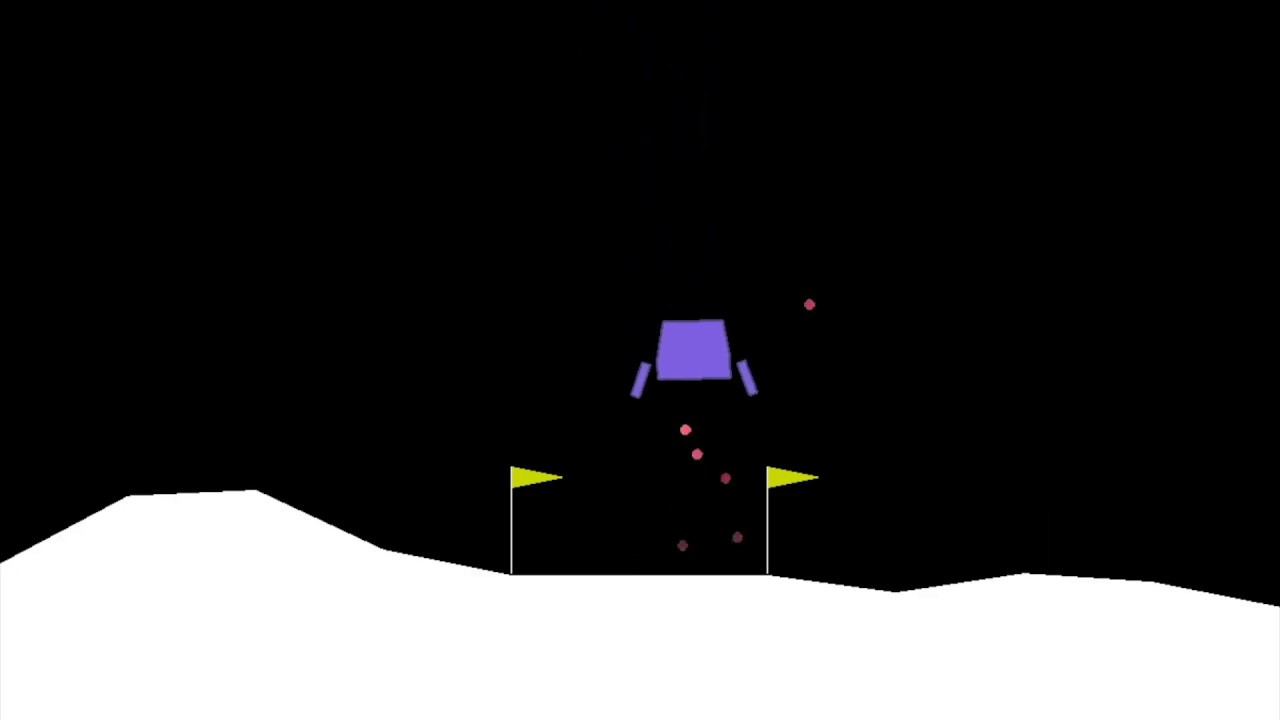
\includegraphics[width=1.5cm]{R.jpeg}};
    % Quadrado esquerdo
    \draw[fill=blue!30] (-3,0) rectangle (-1,2);
    % Quadrado direito
    % Setas
    \node at (-2, 1) {\tiny Agente};
    \node at (3, 0.25) {\tiny Ambiente};
    \draw[->, color=red] (3.5,2) to[out=135, in=45] (-2.5,2);
    \draw[->, color=darkgreen] (2.5,2) to[out=135, in=45] (-1.5,2);
    \draw[->, color=blue] (-2,0) to[out=-45, in=-135] (3,0);
     \node[blue] at (0.5,-.7) {\tiny Ação};
    \node[red] at (0.5, 3.65) {\tiny Recompensa};
    \node[darkgreen] at (0.5, 2.25) {\tiny Observação};
\end{tikzpicture}
\label{fig:loopgym}
\end{figure}
\vspace*{-0.775cm}
{\raggedright \fonte{Autor.}}


Esse processo continua em um loop até que um critério de término seja alcançado, encerrando assim o episódio e garantindo uma interação contínua entre o agente e o ambiente de simulação.

\subsection{\textit{Cart Pole}}
\label{sec:AE}

Neste cenário, o pêndulo é posicionado verticalmente sobre o carrinho, tendo como meta equilibrar o pêndulo ao aplicar forças nas direções esquerda e direita no carro \cite{cartpole}. O \textit{Cart Pole} é um problema clássico que envolve um pêndulo invertido, como representado na Figura \ref{fig:GPC1}.

\begin{figure}[H]
    \centering
    \vspace*{-0.25cm}
    \caption{\textit{Cart Pole}.}
    \animategraphics[width=.35\textwidth, loop, autoplay]{30}%frame rate
    {CPSC.png/10064094-80f5-4740-bbfb-425e476c87c0-}%path to figures
    {0}%start index
    {24}%end index
    \label{fig:GPC1}
\end{figure}
\vspace*{-.8cm}
{\raggedright \fonte{Autor.}}

A interação do \textit{Cart Pole} com algoritmo se dá por meio de sua entrada, conforme ações apresentadas na Tabela \ref{tab:intcartpole1}.

\begin{table}[H]
	\centering
	\vspace*{-0.2cm}
	\caption{Entrada do \textit{Cart Pole}.}
	\begin{tabular}{|c|c|}
            \hline
            Número & Ação  \\
            \hline
            0 & Empurre o carrinho para à esquerda \\
            \hline
            1 & Empurre o carrinho para à direita \\
            \hline
	\end{tabular}  
    \label{tab:intcartpole1}                 % Nome da tabela para referência cruzada
\end{table}
\vspace*{-0.7cm}
{\raggedright \fonte{Autor, adaptado de \cite{gymcartpole}.}}

O espaço de observação constitui a saída, e essas informações são utilizadas para a aplicação de ações futuras de acordo com o espaço de observação da Tabela \ref{tab:outcartpole}.

\begin{table}[H]
	\centering
	\vspace*{-0.2cm}
	\caption{Espaço de observação do \textit{Cart Pole}.}
        \begin{tabular}{|c|c|c|c|}
            \hline
            Número & Observação & Mínimo & Máximo  \\
            \hline
            0 & Posição do carrinho & -4,8 & 4,8\\
            \hline
            1 & Velocidade do carrinho & -Inf & Inf\\
            \hline
            2 & Ângulo do polo &  -0,418 rad (-24°) & 0,418 rad (24°)\\
            \hline
            3 & Velocidade angular do polo & -Inf & Inf\\
            \hline
    \end{tabular}  
    \label{tab:outcartpole}                 % Nome da tabela para referência cruzada
\end{table}
\vspace*{-0.7cm}
{\raggedright \fonte{Autor, adaptado de \cite{gymcartpole}.}}

O ambiente se encerra quando o \textit{Cart Pole} atinge 500 etapas.

\subsection{\textit{Lunar Lander}}
\label{sec:LL}

Neste ambiente, a tarefa consiste em realizar um pouso suave de uma sonda espacial na superfície lunar, lidando com desafios como a gravidade lunar, obstáculos e utilizando informações cruciais, como a posição, ângulo e velocidade da nave, conforme a Figura \ref{fig:GPC1}.

\begin{figure}[H]
    \centering
    \vspace*{-0.25cm}
    \caption{\textit{Lunar Lander}.}
    \animategraphics[width=.41\textwidth, loop, autoplay]{30}%frame rate
    {LLSC.png/1d08ba8c436d45c4836197d017e10367pXCEhE5SPawIdiCa-}%path to figures
    {0}%start index
    {118}%end index
    \label{fig:GPC1}
\end{figure}
\vspace*{-.725cm}
{\raggedright \fonte{Autor.}}

A interação do LunaLander com algoritmo se dá por meio de suas entradas, como mostrado na Tabela \ref{tab:intlunarlander}.

\begin{table}[H]
	\centering
	\vspace*{-0.2cm}
	\caption{Entradas do \textit{Lunar Lander}.}
        \begin{tabular}{|c|c|}
        	 \hline
             Número & Ação\\
             \hline
            0 & Não fazer nada \\
            \hline
            1 & Motor de orientação à esquerda da sonda \\
            \hline
            2 & Acionamento do motor principal\\
            \hline
            3 & Motor de orientação à direita da sonda \\
            \hline
            \end{tabular} 
        \label{tab:intlunarlander}                 % Nome da tabela para referência cruzada
    \end{table}
\vspace*{-.655cm}
{\raggedright \fonte{Autor, adaptado de \cite{gymlunarlander}.}}

Espaço de observação do \textit{Lunar Lander} é composto pelos itens da Tabela \ref{tab:outlunarlander}.

\begin{table}[H]
	\centering
	\vspace*{-0.2cm}
	\caption{Espaço de observação do LunarLander.}
        \begin{tabular}{|c|c|c|c|}
        	\hline
              Número & Observação & Mínimo & Máximo\\
             \hline
            0 & Coordenada x & -1,5 & 1,5\\
            \hline
            1 & Coordenada y & -1,5 & 1,5\\
            \hline
            2 & Velocidade linear em x &  -5 & 5\\
            \hline
            3 & Velocidade linear em y &  -5 & 5\\
            \hline
            4 & Ângulo & -$\pi$  $(-180^\circ)$ & $\pi$ $(180^\circ)$\\
            \hline
            5 & Velocidade angular &  -5 & 5\\
            \hline
            6 & Contato pé esquerdo &  0 & 1\\
            \hline
            7 & Contato pé direito &  0 & 1\\
        \hline
        \end{tabular}
        \label{tab:outlunarlander}                 % Nome da tabela para referência cruzada
    \end{table}
\vspace*{-.655cm}
{\raggedright \fonte{Autor, adaptado de \cite{gymlunarlander}.}}


Após cada passo no jogo \textit{Lunar Lander}, uma recompensa é concedida ao controlador, e a recompensa total de um episódio é a soma dessas recompensas ao longo de todas as etapas do episódio. A recompensa por etapa é determinada pela proximidade do módulo de pouso à plataforma de pouso, pela velocidade do módulo de pouso, pelo ângulo de inclinação do módulo de pouso e pelo número de pernas em contato com o solo. Além disso, há penalidades para o uso dos motores laterais e do motor principal. O episódio também recebe uma recompensa adicional de -100 ou +100 pontos por bater ou pousar com segurança, respectivamente. Um episódio é considerado uma solução se marcar pelo menos 200 pontos.

\section{Método de Pesquisa em Grade}
\label{sec:MPG}

Como discutido, os ambientes têm entradas inteiras, o que sugere a minimização de uma função custo por meio de otimização inteira. Dada a quantidade limitada de entradas, o Método de Pesquisa em Grade é viável. Apesar de uma complexidade \(O(n!)\), indicando crescimento fatorial do tempo de execução devido a $n$, sua aplicação é factível para horizontes de controle mais curtos. Este método examina todas as combinações possíveis de variáveis, evitando convergir erroneamente para mínimos/máximos locais ao buscar o valor mínimo/máximo de uma função.

\section{ Algoritmo Subida de Encosta)}
\label{sec:Hill}

O Método de Subida de Encosta é um algoritmo clássico para otimização \cite{hill}, mostrando-se altamente eficaz na identificação de máximos ou mínimos locais. No processo desse algoritmo, inicia-se a partir de um ponto aleatório $X$ e realiza-se sua avaliação. Em seguida, ocorre o deslocamento do ponto original X para um novo ponto vizinho, designado como $X'$. Se o novo ponto $X'$ representar uma solução superior à do ponto anterior, permanece-se nele e o processo é repetido. Caso não encontre tal aprimoramento, a execução é interrompida.\\
			 
%%%%%%%%%%%%%%%%%%%%%%%%%%%%%% METODOLOGIA (OBRIGATÓRIO) %%%%%%%%%%%%%%%%%%%%%%%%%%%%%%
		
{\let\clearpage\relax\par \chapter{METODOLOGIA}}
\label{ch:metodologia}                      % Nome do capítulo para referência cruzada

% ===========================================================
\section{Considerações Iniciais}
\label{sec:considIniciaisMetodologia}               % Nome da seção para referência cruzada

A elaboração da metodologia incorporou a totalidade do conteúdo abordado na \hyperref[ch:conceitosPreliminares]{Seção de Conceitos Preliminares}, englobando também a modelagem de sistemas dinâmicos por meio de equações diferenciais e modelos ARX. Na implementação foram utilizados pacotes na linguagem Python, destacando-se o Gymnasium, SysIdentPy e GEKKO.


% ===========================================================
\section{\textit{Cart Pole}: Implementação e Sintonia do Controlador PID}
\label{sec:pidcartpole}                     % Nome da seção para referência cruzada

Nesta seção, é abordada a implementação do controlador PID para o \textit{Cart Pole}.

\subsection{Obtenção da Função de Transferência para o \textit{Cart Pole}}
\label{subsec:titprov}                     % Nome da seção para referência cruzada

O primeiro ambiente a ser abordado é o \textit{Cart Pole}, o primeiro passo é obter a sua FT, conforme discutido por Ogata \cite{ogata2010engenharia}. Este passo é crucial para a subsequente implementação do controlador PID, visando controlar o sistema \textit{Cart Pole} \cite{cpepid}. O sistema em questão refere-se a um pêndulo invertido montado em um carro motorizado, como mostrado na Figura \ref{fig:penduloinvertido}.

\begin{figure}[H]
    \centering
    \vspace*{-0.2cm}
    \caption{Sistema de pêndulo invertido.}
    \begin{tikzpicture}[every node/.style={font=\footnotesize}]
    % Cartpole 1
        \draw[pattern=north east lines, pattern color=black,  draw=white] (-0.1,0) rectangle (6,-0.1);
        \draw[pattern=north east lines, pattern color=black,  draw=white] (0,0) rectangle (-0.1,1.3);
        \draw (0,0) -- (6,0);
        \draw (0,0) -- (0,2.6);
        \draw (2.4, 0.15) circle (0.15cm);
        \draw (3.6, 0.15) circle (0.15cm);
        \draw (2,0.3) -- (4,0.3) -- (4,1.3) -- (3.2,1.3);
        \draw(2.8,1.3)--(2,1.3)--node[right]{$M$}(2,0.3);
        \draw (3.2,1.3) arc (0:180:0.2cm);
        \draw (2.95, 1.3)--(3.6, 3);
        \draw (3.05, 1.3)--(3.7, 3);
        \draw (3.05,1.3) arc (0:-180:0.05cm);
        \draw (3.7,3) arc (0:180:0.05cm);
        \filldraw[black] (3,1.3) circle (0.02cm);
        \draw[->](0,2.6)--node[above left]{$y$}(0,3.2);
        \draw (0, 1.3)--(2.8, 1.3);
        \draw (4, 1.3)--(4.5, 1.3);
        \draw[->](4.5,1.3)--node[above left]{$x$}(4.7,1.3);
        \draw (3, 1.3)--(3, 3);
        \draw [->](3,2.7) arc (150:62:0.4cm) node[above left]{$\theta$};
        \draw[<->](0,2.65)--node[above left]{$x$}(3,2.65);
        \draw[->] (1.5,0.8) -- (2,0.8) node[above left] {$u$};
        \draw (2, 2.15)--(3.32, 2.15);
        \draw[<->](2.3,1.3)--node[midway, left]{$\ell\:cos\theta$}(2.3,2.15);
        \draw[->](3.32,2.15)--node[pos=2, above]{$\:\:mg$}(3.32,1.75);
        \draw[<->](3.6,1.033)--node[right]{$\ell$}(3.95,1.883);
        \draw (3.05, 1.2445)--(3.6, 1.033);
        \draw (3.4, 2.138)--(3.95, 1.883);
        \draw (3.74, 3)--(4.29, 2.783);
        \draw [<->](3.95, 1.883)--node[right]{$\ell$}(4.29, 2.783);
        \node  at (-0.2,1.3) {$O$};
        \node  at (3,1) {$P$};
    \end{tikzpicture}
    \label{fig:penduloinvertido}
\end{figure}
\vspace*{-0.8cm}
{\raggedright \fonte{Autor, adaptado de \cite{ogata2010engenharia}.}}

O primeiro passo é modelar o sistema de pêndulo invertido, a ideia é encontrar como a entrada é dinamicamente transferida para a saída, encontrando a FT do sistema, que para o sistema pêndulo invertido a entrada é a força aplicada na lateral ($u$) e a saída o ângulo do pêndulo ($\theta$), conforme a Figura \ref{fig:sys}.

Para deduzir as equações de movimento do sistema, foi realizado o estudo do diagrama de corpo livre do sistema de pêndulo invertido, conforme ilustrado na Figura \ref{fig:corpolivre}:

\begin{figure}[H]
    \centering
    \vspace*{-0.2cm}
    \caption{Diagrama de corpo livre do pêndulo invertido.}
    \begin{tikzpicture}[every node/.style={font=\footnotesize}]
        \draw[pattern=north east lines, pattern color=black,  draw=white] (-0.1,0) rectangle (6,-0.1);
        \draw[pattern=north east lines, pattern color=black,  draw=white] (-0.1,-0.1) rectangle (0,1.3);
        \draw (0,0) -- (6,0);
        \draw (0,0) -- (0,1.3);
        \draw (2.4, 0.15) circle (0.15cm);
        \draw (3.6, 0.15) circle (0.15cm);
        \draw (2,0.3) -- (4,0.3) -- (4,1.3) -- (3.2,1.3);
        \draw(2.8,1.3)--(2,1.3)--node[right]{$M$}(2,0.3);
        \draw (3.2,1.3) arc (0:180:0.2cm);
        \draw (3, 1.6)--(3.65, 3);
        \draw (3.1, 1.6)--(3.75, 3);
        \draw (3.1,1.6) arc (0:-180:0.05cm);
        \draw (3.75,3) arc (0:180:0.05cm);
        \draw[->](0,2.6)--node[above left]{$y$}(0,3.2);
        \draw(0,1.3)--(0,2.6);
        \draw (3, 2.25)--(3,3);
        \draw [<->] (0, 2.75)--node[above left]{$x$}(3, 2.75);
        \draw [->](3,2.6) arc (150:55:0.35cm) node[above left]{\small $\theta$};
        \draw[->](3.375,2.3)--node[pos=2, above]{$\:\:mg$}(3.375,1.9);
        \draw[->] (1.5,0.8) -- (2,0.8) node[above left] {$u$};
        %\draw (3.03, 1.557)--(3.72,3.042);
        %\draw (2.88, 1.626)--(3.57,3.111);
        \draw (2.655,2.6248)--(3.225,2.3688);
        \draw [<->](2.33, 1.882)--node[left]{$\ell$}(2.655,2.6248);
        \draw [<->](2.655,2.6248)--node[left]{$\ell$}(2.972,3.367);
        \draw (3.57,3.111)--(2.972,3.367);
        \draw (2.33, 1.882)--(2.88, 1.626);
        \draw[->, blue] (2.98,1.535) -- (2.48,1.535) node[left] {$H$};
        \draw[->, blue] (2.98,1.535) -- (2.98,1.03) node[left] {$V$};
        \draw[->, red] (2.9875,1.54) -- (2.9875,2.05) node[left] {$V$};
        \draw[->, red] (2.9875,1.54) -- (3.4875,1.54) node[right] {$H$}; 
    \end{tikzpicture}
    \label{fig:corpolivre}
\end{figure}
\vspace*{-0.8cm}
{\raggedright \fonte{Autor, adaptado de \cite{ogata2010engenharia}.}}

O deslocamento horizontal do carro é descrito pela Equação \ref{eq:hori}:

\begin{equation}
    \label{eq:hori}
    M\frac{d^2x}{dt} = u - H.
\end{equation}

Já o deslocamento do centro de massa do pêndulo ($x_c$) é ilustrado na Figura \ref{fig:des}:

\begin{figure}[H]
    \definecolor{lightbrown}{RGB}{205,133,63} % Define a cor marrom claro
    \centering
    \vspace*{-0.2cm}
    \caption{Deslocamento do centro de massa do pêndulo.}
    \begin{tikzpicture}[every node/.style={font=\footnotesize}]
         % Cartpole 1
        \draw [->](-3, 0) --node[above left]{$y$}(-3, 1);
        \draw [->](-3, 0) --node[above right]{$x$}(-2, 0);
        \draw[fill = lightbrown, rotate around={0:(0,0)}]  (0,0) rectangle (0.1,3);
        \node[circle,fill=green,inner sep=1pt] at (0.05,1.5) {};
        \draw[fill = lightbrown, rotate around={-45:(0,0)}] (0,0) rectangle (0.1,3);
        \node[circle,fill=cyan,inner sep=1pt] at (1.0606,0.986) {};
        \coordinate (A) at (1.13,1);
        \coordinate (B) at (-.2,-.2);
        \coordinate (C) at (0.11,1);
        \draw (-0.1, 0) -- (-1.2,0);
        \draw (-0.1, 1.5) -- (-1.2,1.5);
        \draw [<->, fill=black](-1.15, 0)--node[left]{$\ell$} (-1.15,1.5);
        \draw [<->](0.05, 0.986)--node[above]{$\ell sen\theta$} (1.0606,0.986);
        \draw (-0.1, 0.986) -- (-0.2,0.986);
        \draw [<->](-0.15, 0) --node[left]{$\ell cos\theta$}(-0.15,0.986);
        \draw[dashed] (0.05,1.5) -- (2,1.5); 
        \draw[dashed] (1.0606,0.986) -- (2,0.986); 
        \draw [<->](1.95, 0.986) --node[right]{$\ell - \ell cos\theta$}(1.95, 1.5);
        \pic[draw=black, <->, angle radius=1cm, angle eccentricity=.8]{angle = A--B--C};
        \node at (.225,.5) {$\theta$};
    \end{tikzpicture}
    \label{fig:des}
\end{figure}
\vspace*{-0.7cm}
{\raggedright \fonte{Autor, adaptado de \cite{ogata2010engenharia}.}}

Na Figura \ref{fig:des}, observa-se que a coordenada $x_c$ do carro é obtida pela soma do deslocamento horizontal do centro de massa da coordenada que se encontra, representado como $x_c=x + \ell\:\sin\theta$, e tomando a segunda derivada de $x_c$ efetuando o balanço das forças horizontais, encontra-se a Equação \ref{eq:descmh}:

\begin{equation}
    m\frac{d^2}{dt}(x+\ell\:sen\theta) = H.
    \label{eq:descmh}
\end{equation}

O $y_c$ pode ser encontrado subtraindo $\ell\:cos\theta$ de $\ell$, agora, basta tomar a sua segunda derivada igual à resultante de forças verticais ($mg-V$):

\begin{equation}
    m\frac{d^2}{dt}(\ell-\ell\:cos\theta) = mg - V.
    \label{eq:descmv}
\end{equation}

No entanto, como $\ell$ é uma constante e sua segunda derivada é zero, a Equação \ref{eq:descmv} pode ser reformulada conforme a Equação \ref{eq:descmvref}:

\begin{equation}
    m\frac{d^2}{dt}(-\ell\:cos\theta) = mg - V \Longrightarrow  m\frac{d^2}{dt}(\ell\:cos\theta) = V-mg.
    \label{eq:descmvref}
\end{equation}

O próximo passo consiste em determinar o deslocamento rotacional, conforme mostrado na Figura \ref{fig:desr}.

\begin{figure}[H]
    \definecolor{lightbrown}{RGB}{205,133,63} % Define a cor marrom claro
    \centering
    \vspace*{-0.2cm}
    \caption{Deslocamento rotacional do centro de gravidade do pêndulo,}
    \begin{tikzpicture}[every node/.style={font=\footnotesize}]
        % Cartpole 1
        \draw[rotate around={0:(0,0)}]  (0,1.45) rectangle (0.1,-1.45);
        \draw[fill = lightbrown, rotate around={-45:(0,0)}]  (0,1.5) rectangle (0.1,-1.5);
        \node[circle,fill=blue,inner sep=1pt] at (0.05,0) {};
        \draw [->, red](-1.015, -1.1) --node[above right]{$V$}(-1.015, 0.015);
        \draw [->, red](-1.015, -1.1) --node[above right]{$H$}(-0.015, -1.1);
        \draw [->, orange](-1.015, 0.015) --node[above left]{$V\:cos\theta$}(-1.515, -0.5153);
        \draw [->, orange](-0.015, -1.1) --node[below right]{$H\:sen\theta$}(-0.545, -1.63);
        \draw [->, orange](-1.015,-1.1) --node[below left]{$H\:cos\theta$}(-0.545, -1.63);
        \draw [->, orange](-1.015, -1.1) --node[below left]{$V\:sen\theta$}(-1.515, -0.5153);
    \end{tikzpicture}
    \label{fig:desr}
\end{figure}
\vspace*{-0.9cm}
{\raggedright \fonte{Autor, adaptado de \cite{ogata2010engenharia}.}}

O movimento rotacional da haste do pêndulo ao redor de seu centro de gravidade é descrito pela Equação \ref{eq:rot}:

\begin{equation}
    I\frac{d^2\theta}{dt} = V\ell\:sen\theta - H\ell\:cos\theta,
    \label{eq:rot}
\end{equation}

\noindent onde $I$ representa o momento de inércia da haste em relação ao centro de gravidade.

As Equações \ref{eq:hori}, \ref{eq:descmh}, \ref{eq:descmvref} e \ref{eq:rot} descrevem o comportamento dinâmico do pêndulo invertido. No entanto, essas equações envolvem funções trigonométricas, como seno e cosseno. Para linearizá-las, foi adotado um valor muito pequeno para $\theta$. A ideia é manter o sistema estável, permitindo assim aproximações úteis, tais como:  $cos\theta \approx 1$ e $sen\theta \approx \theta$. Portanto:

\begin{equation}
    I\frac{d^2\theta}{dt} = V\ell\theta - H\ell,
    \label{eq:rots}
\end{equation}

\begin{equation}
    M\frac{d^2x}{dt} = u - H,
    \label{eq:horis}
\end{equation}

\begin{equation}
    m\frac{d^2}{dt}(x+\ell\theta) = H,
    \label{eq:descmhs}
\end{equation}

\begin{equation}
    m\frac{d^2}{dt}(\ell) = V - mg\Longrightarrow  0 = V-mg.
    \label{eq:descmvs}
\end{equation}

Note que $H$ e $V$ são desconhecidos, mas \textit{a priori} não se trata de um problema, pois pela Equação \ref{eq:descmhs} é possível expressar $H$. Pela Equação \ref{eq:descmvs}, tem-se que $V = mg$, levando ao próximo passo, substituir esses valores na Equação \ref{eq:rots}, obtendo:

\begin{equation}
    I\frac{d^2\theta}{dt} = mg\theta\ell-m \frac{d^2}{dt} (x+\ell\theta)\ell.
    \label{eq:HeV}
\end{equation}

Ao igualar a zero, tem-se:

\begin{equation}
    (I + m\ell^2)\frac{d^2\theta}{dt^2} + m\ell\frac{d^2x}{dt^2} - mg\ell\theta = 0.
    \label{eq:HeV0}
\end{equation}

Substituindo a Equação \ref{eq:descmhs} na Equação \ref{eq:horis}, obtém-se:

\begin{equation}
    M\frac{d^2x}{dt^2}  = u -  m\frac{d^2}{dt^2} (x + \ell\theta).
    \label{eq:Id2r}
\end{equation}

Reorganizando os termos:

\begin{equation}
    M\frac{d^2x}{dt^2} + m\frac{d^2}{dt^2} (x + \ell\theta) = u.
    \label{eq:Id2r}
\end{equation}

Agora, é necessário obter a função de transferência do sistema. Logo, naturalmente, é preciso transformar as Equações \ref{eq:HeV0} e \ref{eq:Id2r} para o domínio de Laplace com condições iniciais nulas, conforme segue:

\begin{equation}
    (I + m\ell^2)s^2\Theta(s) + m\ell s^2 X(s) - mg\ell\Theta(s) = 0,
    \label{eq:L1}
\end{equation}

\begin{equation}
    (M+m)s^2 X(s) + m\ell s^2\Theta(s) = U(s).
    \label{eq:L2}
\end{equation}

A ideia volta-se para obter a relação da saída ($\Theta (s)$) em relação à entrada ($U(s)$). Portanto, o $X(s)$ deve ser eliminado. Considerando a Equação \ref{eq:L1}, tem-se:

\begin{equation}
    ((I + m\ell^2)s^2 - mg\ell)\Theta(s) + m\ell s^2 X(s) = 0.
    \label{eq:L3}
\end{equation}

Isolando $X(s)$, a Equação \ref{eq:L3} pode ser reescrita como:

\begin{equation}
    X(s) = -\frac{\{(I+m\ell^2)s^2-mg\ell\}}{m\ell s^2} \Theta (s),
    \label{eq:X}
\end{equation}

\noindent substituindo a Equação \ref{eq:X} na Equação \ref{eq:L2}, chega-se a:

\begin{equation}
    \begin{split}
        -(M+m)\cancel{s^2} \frac{\{(I+m\ell^2)s^2-mg\ell\}}{m\ell \cancel{s^2}} \Theta (s) + m\ell s^2\Theta(s) = U(s),\\
        \frac{[m^2\ell^2 s^2 - (M+m)\{(I+m\ell^2)s^2-mg\ell\}]}{m\ell}\Theta (s) = U(s).
    \end{split}
    \label{eq:TF1}
\end{equation}

Por fim, tem-se a FT:

\begin{equation}
    \frac{\Theta (s)}{U(s)} = \frac{m\ell}{(m^2\ell^2-(M+m)(I+m\ell^2))s^2+(M+m)mg\ell}.
    \label{eq:TF}
\end{equation}

Ainda é necessário saber quais são os valores de massa, comprimento e momento de inércia. Na verdade, não é preciso conhecer o valor exato de cada uma dessas grandezas, pode-se aproximá-las com simulações e um pouco de física. Portanto, será aplicada uma força à direita (aplicar 1 a entrada, conforme a Tabela \ref{tab:intcartpole}) para observar como o sistema se comporta. Como o ambiente fornece os valores de velocidade e velocidade angular, é possível plotá-los para encontrar alguns valores para as variáveis supracitadas, como mostrado na Figura \ref{fcte}.

\begin{figure}[H]
     \centering
     \vspace*{-0.2cm}
     \caption{Resultados da aplicação de uma força constante à direita.}
     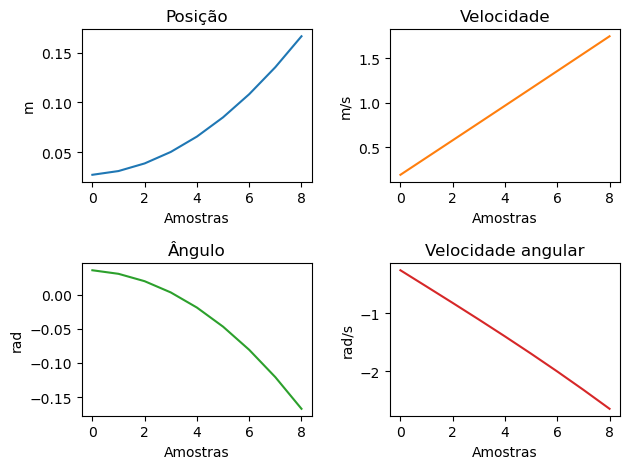
\includegraphics[scale=.55]{Grafico1.png}
     \label{fcte}
\end{figure}
\vspace*{-0.8cm}
{\raggedright \fonte{Autor, adaptado de \cite{cpepid}.}}

Não se pode realmente obter muitas informações úteis da posição ou ângulo, mas o fato de que a velocidade e a velocidade angular serem lineares é muito importante. Isso sugere que a simulação é fisicamente precisa, pois uma força constante está produzindo uma aceleração constante tanto linear quanto angularmente, conforme descrito pela Segunda Lei de Newton.


As acelerações linear e angular correspondem à inclinação da velocidade, representada como uma reta linear. Para calcular essas inclinações, foi utilizada a função linregress do pacote Scipy. Os resultados obtidos foram:

\begin{equation}
    \begin{matrix}
        \ddot{x} = 0,19524\frac{m}{s^2} & \text{e} & \ddot{\theta} =-0,29775\frac{rad}{s^2}.
    \end{matrix}
\label{eq:vlevt}
\end{equation}

Um fato interessante, é que esses valores permanecem constantes, independentemente do número de simulações, sugerindo que o ambiente \textit{Cart Pole} possui um embasamento físico subjacente. Considere a Figura \ref{fig:cartPole}.

\begin{figure}[H]
    \definecolor{lightbrown}{RGB}{205,133,63} % Define a cor marrom claro
    \centering
    \vspace*{-0.2cm}
    \caption{\textit{Cart Pole}.}
    \centering 
    \begin{tikzpicture}[scale=0.8, every node/.style={font=\tiny}]
        % Cartpole 1
        \draw[fill=black] (0,0) rectangle (0.75,0.5);
        \draw[fill=black] (-2,.25) -- (3,.25);
        \draw[fill = lightbrown, rotate around={75:(0.565,0.1)}] (0.5,0.25) rectangle (2,0.385);
        \node[circle,fill=purple,inner sep=1pt] at (0.375,0.25) {};
        \draw [->, blue] (-.5,0.025) -- node[left]{$\Vec{F}$ à direita\:\:}(0, 0.025);
        \coordinate (A) at (.4,.55);
        \coordinate (B) at (.35,.35);
        \coordinate (C) at (0,.55);
        \pic[draw=green, ->, angle radius=1cm,angle eccentricity=.2] {angle = A--B--C};
        %\draw [-, violet] (0.45,1.65) -- node[below left]{$\tau$}(0.45, 1.65);
        \node[color=black] at (1.5,1) {\large $I>0$};
    \end{tikzpicture}
    \label{fig:cartPole}
\end{figure}
\vspace*{-0.8cm}
{\raggedright \fonte{Autor, adaptado de \cite{gymcartpole}.}}

O momento de inércia deve ser sempre positivo, conforme a Figura \ref{fig:cartPole}. Para tal análise, foi utilizada a Equação \ref{eq:an1}:

\begin{equation}
    (I + m\ell^2)\frac{d^2\theta}{dt^2} + m\ell\frac{d^2x}{dt^2} - mg\ell\theta = 0.
    \label{eq:an1}
\end{equation}

Como o intuito é mantê-lo equilibrado, $\theta \approx 0$, abrindo a possibilidade de reescrever a Equação \ref{eq:an1} da seguinte forma:

\begin{equation}
    (I + m\ell^2)\frac{d^2\theta}{dt^2}   = - m\ell\frac{d^2x}{dt^2},
    \label{eq:an22}
\end{equation}

\noindent onde $\frac{d^2\theta}{dt^2} = -0,29775\frac{rad}{s^2}$ e $\frac{d^2x}{dt^2} = 0,19524\frac{m}{s^2}$, o valor adotado para $m$ será $0,5 kg$. Logo:

\begin{equation}
    I = \frac{0,0976\ell - 0,1488\ell^2}{0,29775}.
    \label{eq:an2}
\end{equation}

A Equação \ref{eq:an2} expressa $I$ em função de $\ell$. Ao variar $\ell$ de $0$ a $1m$, obtém-se o Gráfico \ref{miec}.

\begin{figure}[H]
     \centering
     \vspace*{-0.2cm}
     \caption{Relação entre momento de inércia e o comprimento, para $m=0,5kg$.}
     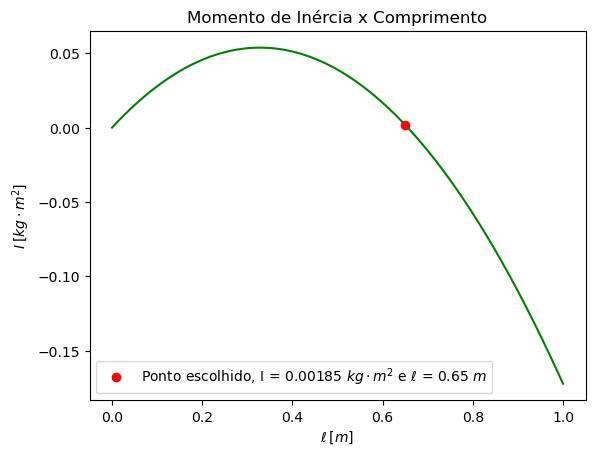
\includegraphics[scale=.55]{Grafico2.png}
     \label{miec}
\end{figure}
\vspace*{-.85cm}
{\raggedright \fonte{Autor.}}

Note que o valor escolhido de $\ell$ apresenta $I$ positivo.

O próximo passo consiste em estimar a massa do carro  (\(M\)) utilizando a Equação \ref{eq:M}:

\begin{equation}
    (M + m)\frac{d^2 x}{dt^2} + m\ell \frac{d^2 \theta}{dt^2} = u.
    \label{eq:M}
\end{equation}

Substituindo os valores conhecidos, como $m = 0,5kg$, $u = 1N$ e $\ell = 0,65m$, obtém-se:

\begin{equation}
    M = \frac{u - m\ell\ddot{\theta}-m\ddot{x}}{\ddot{x}} = \frac{1 + 0,5\cdot 0,65\cdot 0,29775 - 0,5\cdot 0,19524}{0,19524} = 5,11754 kg.
    \label{eq:Mn}
\end{equation}


Os resultados obtidos ou definidos estão apresentados na Tabela \ref{tab:paramct}.


\begin{table}[H]
	\centering
	\vspace*{-0.2cm}
	\caption{Valores dos parâmetros.}
    \begin{tabular}{|c|c|c|c|}
    		\hline
            $M [kg]$ & $m [kg]$ & $\ell [m]$ & $I[kg\cdot m^2]$\\
            \hline
            $5,11754$ & $0,5$ & $0,65$ & $1,8537\times 10^{-3}$ \\
            \hline
        \end{tabular}
        \label{tab:paramct}                 % Nome da tabela para referência cruzada
 \end{table}
\vspace*{-0.675cm}
{\raggedright \fonte{Autor.}}

Ao substituí-los na Função de transferência da Equação \ref{eq:TF}, chega-se:

\begin{equation}
     \frac{\Theta (s)}{U(s)} = \frac{0,325}{-1,0914s^2 + 17,9101}.
    \label{eq:FT1}
\end{equation}

A função de transferência faz sentido a priori, pois uma força para a direita deve resultar em um ângulo $\theta$ negativo. No entanto, é necessário validar a função de transferência com o ambiente \textit{Cart Pole} do Gymnasium. Portanto, ocorreu a aplicação da mesma entrada tanto no ambiente \textit{Cart Pole} quanto na função de transferência, considerando apenas um episódio (até o sistema perder a estabilidade). A cada episódio, o ambiente é reiniciado. Para adequar a entrada, foi empregada a seguinte formulação: no \textit{Cart Pole}, a entrada $1$ significa ir para a direita, enquanto $0$ é o comando para ir à esquerda. Para a função de transferência, o movimento para a direita também é representado por $1$, porém, para a esquerda, é representado por $-1$. Assim, tem-se o gráfico da Figura \ref{fig:entvalft1}.

\begin{figure}[H]
     \centering
     \vspace*{-0.2cm}
     \caption{Entrada e saída.}
     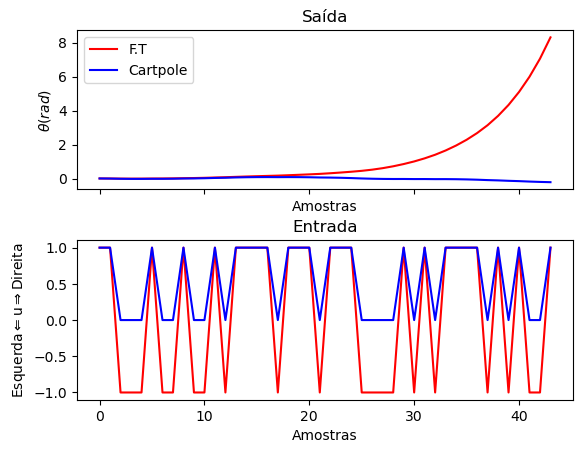
\includegraphics[scale=.53]{entval.png}
     \label{fig:entvalft1}
\end{figure}
\vspace*{-.85cm}
{\raggedright \fonte{Autor.}}


A partir da Figura \ref{fig:entvalft1}, nota-se que a FT não conseguiu representar o sistema adequadamente. A FT responde de forma muito lenta aos estímulos de entrada. Portanto, é necessário ajustá-la para obter respostas mais abruptas. Ao observar os passos anteriores, a aceleração considerada levou em conta $8$ amostras, com um intervalo de $1s$ entre amostras, para realmente encontrar a inclinação. No entanto, devido à natureza computacional, o tempo é significativamente menor. Assim, as acelerações em $x$ e angular serão multiplicadas por um fator ($k$) até que a FT alcance um desempenho satisfatório. Dessa forma, será retornado a equação da inércia:

\begin{equation}
    (I + m\ell^2)\frac{d^2\theta}{dt^2}\cancel{k}   = - m\ell\frac{d^2x}{dt^2} \cancel{k},
    \label{eq:inercia}
\end{equation}

\noindent logo, o momento de inércia independe do valor de \(k\). Portanto, os valores de \(I\) e \(\ell\) permanecem inalterados, sendo \(1,8537\times 10^{-3} N\cdot m\) e \(0,65 m\), respectivamente.

De acordo com a teoria, à medida que a aceleração aumenta enquanto a força permanece constante, espera-se que a massa total ($M+m$) diminua. Em termos matemáticos, isso é evidenciado pela Equação \ref{eq:Ma}, onde $m$ é mantido constante em $0,5 kg$ (Massa do pêndulo), resultando em uma diminuição de $M$ (Massa do carro), conforme descrito a seguir:

\begin{equation}
    M = \frac{u - k\:m\ell\ddot{\theta}-k\:m\ddot{x}}{k\ddot{x}}.
    \label{eq:Ma}
\end{equation}

Um aspecto crucial a ser considerado é que a massa do carrinho deve ser um valor positivo ($M > 0$). Portanto:

\begin{equation}
    0 < \frac{u - k\:m\ell\ddot{\theta}-k\:m\ddot{x}}{k\ddot{x}} \Rightarrow 0 < 1 + k\cdot 0,5\cdot 0,65\cdot 0,29775-k\cdot 0,5\cdot 0,19524.
    \label{eq:M>0}
\end{equation}

Ao resolver a Inequação \ref{eq:M>0}, chega-se a $k<1174,74$, logo, para determinar o valor de \( k \), ele será variado de 1 a 1174, considerando 1000 etapas (amostras). Um conjunto de etapas compõe o episódio, sendo que cada episódio é concluído quando o ângulo do polo não está mais na faixa de \( \pm 12^\circ \) $(\pm 0,2095rad)$. Conformedemonstrado na Figura \ref{fig:ep}.

\begin{figure}[H]
     \centering
     \vspace*{-.25cm}
     \caption{Episódios inteiros.}
     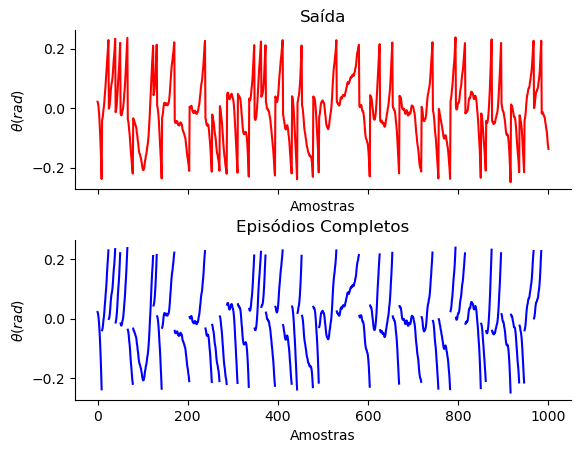
\includegraphics[scale=.53]{episodio.png}
     \label{fig:ep}
\end{figure}
\vspace*{-.8cm}
{\raggedright \fonte{Autor.}}

Ao total, foram realizados 47 episódios completos. Portanto, para cada valor de \(k\), a simulação é repetida 47 vezes, e o somatório do Erro Quadrático Médio (\(RMSE\))\cite{aguirre2004} é calculado. Em seguida, é determinada a média para obter o \(RMSE\) médio associado a \(k\), da seguinte forma:

\begin{equation}
    \overline{RMSE}_k = \frac{1}{47} \sum_{ep=1}^{47} \frac{\sqrt{\sum_{i=1}^{N}(y_{ep}(i)-\hat{y}_{ep}(i))^2}}{\sqrt{\sum_{i=1}^{N}(y_{ep}(i)-\bar{y}_{ep})^2}},
\label{eq:RMSE}
\end{equation}

\noindent onde $\hat{y}_{ep}(i)$ representa a simulação livre para cada episódio (FT) e ${y}_k$ é o sinal medido para cada episódio, com a média ($\bar{y}_{ep}$) sendo calculada na janela de identificação. O resuldado da Equação \ref{eq:RMSE} será plotado na Figura \ref{fig:R}.

\begin{figure}[H]
     \centering
     \vspace*{-0.25cm}
     \caption{RMSE médio devido ao fator $k$.}
     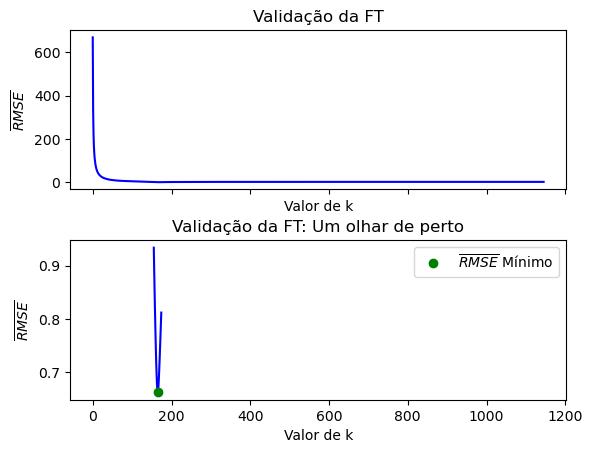
\includegraphics[scale=.53]{RMSE1.png}
     \label{fig:R}
\end{figure}
\vspace*{-.85cm}
{\raggedright \fonte{Autor.}}

Ao empregar o comando \textit{min} do Python, obtém-se um valor de $\overline{RMSE}$ igual a $0,66$ para $k=165$. Ao tomar $k=165$, obtém-se uma FT que responde melhor aos estímulos da entrada. A nova massa a ser:

\begin{equation}
    M = \frac{1 + 165\cdot0,5\cdot0,65\cdot0,29775-165\cdot0,5\cdot0,19524}{165\cdot0,19524} = 0,02668 kg.
    \label{eq:MV}
\end{equation}

Com os novos valores dos parâmetros, a FT passa a ser:

\begin{equation}
     \frac{\Theta (s)}{U(s)} = \frac{0,325}{-0,00661s^2 +  1,67919}.
    \label{eq:31}
\end{equation}

Logo, pode-se representar o diagrama de blocos em malha aberta do sistema conforme a Figura \ref{fig:dbft}.

\begin{figure}[H]
\centering
\vspace*{-.2cm}
\caption{Diagrama do sistema.}
\begin{tikzpicture}[auto, node distance=2cm]
    % We start by placing the blocks
    \node [input, name=input] {};
    \node [block] (system){};
    \draw [->] (-2.5,0) -- node {$U(s)$} (system);
    \draw [->] (system) -- node{$\Theta (s)$} (2.5,0);
    \node [block, pin={[pinstyle]above:Distúrbios},
    node distance=3cm] (system) {$\frac{0,325}{-0,0066s^2 +  1.6792}$};
\end{tikzpicture}
\label{blocos}
\label{fig:dbft}
\end{figure}
\vspace*{-.65cm}
{\raggedright \fonte{Autor.}}

Onde $U(s)$ representa a direção da força com módulo de $1N$ aplicada (com 1 indicando para a direita e -1 para a esquerda), enquanto $\Theta$ refere-se ao ângulo do pêndulo.

Uma abordagem adicional envolve a identificação das raízes do polinômio no denominador da Função de Transferência, que são $15,9351$ e $-15,9351$. É crucial notar que uma destas raízes está localizada no semiplano direito do eixo real, indicando a presença de um sistema instável.

Como exemplo do desempenho da FT, na Figura \ref{fig:dsphft}, uma entrada é aplicada ao sistema para analisar como ele se comporta.

\begin{figure}[H]
     \centering
     \vspace*{-0.2cm}
     \caption{Entrada e saída - Validação da FT.}
     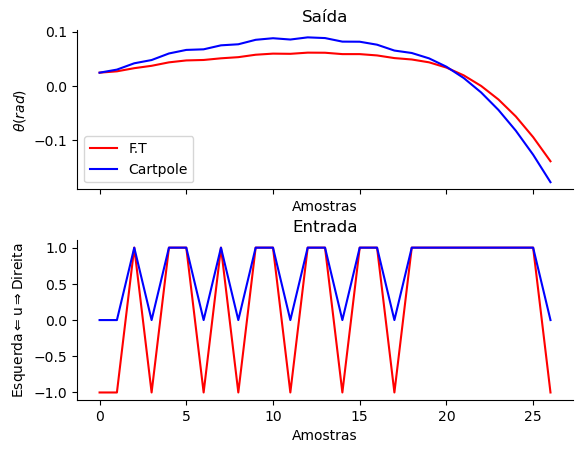
\includegraphics[scale=.575]{entval2.png}
     \label{fig:dsphft}
\end{figure}
\label{fig:entval}
\vspace*{-.8cm}
{\raggedright \fonte{Autor.}}


\subsection{Sintonia do PID}
\label{subsec:sPID}    

Para estabilizar o sistema, foi empregado um controlador PID como ilustrado na Figura \ref{fig:mfpidex}.

\begin{figure}[H]
\centering
\vspace*{-.2cm}
\caption{Malha de controle para o \textit{Cart Pole}.}
% The block diagram code is probably more verbose than necessary
\begin{tikzpicture}[auto, node distance=2.275cm]
    % We start by placing the blocks
    \node [input, name=input] {};
    \node [sum, right of=input] (sum) {};
    \node [block, right of=sum] (controller) {PID};
    \node [block, right of=controller, pin={[pinstyle]above:Distúrbios},
            node distance=3.55cm] (system) {$\frac{0,325}{-0,0066s^2 +  1,6792}$};
    % We draw an edge between the controller and system block to 
    % calculate the coordinate u. We need it to place the measurement block. 
    \draw [->] (controller) -- node[name=u] {$U(s)$} (system);
    \node [output, right of=system] (output) {};
    \node [block, below of=u] (measurements) {Medida do ângulo};

    % Once the nodes are placed, connecting them is easy. 
    \draw [draw,->] (input) -- node {$R(s)$} (sum);
    \draw [->] (sum) -- node[pos=0.44] {$E(s)$} (controller);
    \draw [->] (system) -- node [name=y, pos=0.9] {$Y(s)$}(output);
    \draw [->] (y) |- (measurements);
    \draw [->] (measurements) -| node[pos=0.99] {$-$} 
        node [near end] {$Y_m(s)$} (sum);
\end{tikzpicture}
\label{fig:mfpidex}
\end{figure}
\vspace*{-.7cm}
{\raggedright \fonte{Autor.}}

No âmbito temporal, a formulação da expressão para um controlador PID é delineada da seguinte maneira:

\begin{equation}
     g(t) = K_C \cdot e(t) + \frac{K_C}{\tau_I}\cdot \int_0^t e(t) dt + K_C\cdot \tau_D \cdot \frac{de(t)}{dt}.
    \label{eq:tempopid}
\end{equation}

Para a determinar dos valores de $K_P$, $K_I$ e $K_D$, foi utilizado o pacote GEKKO\cite{gekko}. Este pacote é uma ferramenta em Python dedicada ao aprendizado de máquina e otimização de inteiros mistos, bem como a equações algébricas diferenciais usada para resolver a Equação \ref{eq:tempopid}.Nessa equação, os valores de $\tau_i$ e $\tau_d$ foram ajustados para 2 e 0.25, respectivamente, por meio de tentativa e erro. Em seguida, o pacote fornecerá o valor de $K_C$. A partir desse ponto, os parâmetros podem ser facilmente determinados.A referência consiste em um impulso, representando um distúrbio ideal:

\begin{equation}
     e(t) = r(t) - y_m(t).
    \label{eq:erro}
\end{equation}

O GEKKO, ao buscar a minimização do erro, simplifica o processo, necessitando apenas da introdução da FT e da aplicação do impulso à entrada. Os valores estimados estão vinculados ao $K_C$ determinado, o qual é 0,5, os valores de $\tau_i$ e $\tau_d$ foram previamente estabelecidos como 2 e 0,25. Os valores dos ganhos proporcional, derivativo e integral do PID estão apresentados na Tabela \ref{tab:parcp}.


\begin{table}[H]
	\centering
	\vspace*{-.2cm}
	\caption{Parâmetros do PID.}
        \begin{tabular}{|c|c|c|}
        	\hline
             Termos & Relação com $K_C$ & Valor \\
            \hline
            Proporcional & $K_C$ & 0,5 \\
            \hline
            Integral & $\frac{K_C}{\tau_I}$ & 0,25 \\
            \hline
            Derivativo & $K_C \cdot \tau_D$ & 0,125 \\
            \hline
        \end{tabular}
        \label{tab:parcp}                 % Nome da tabela para referência cruzada
    \end{table}
\vspace*{-0.65cm}
{\raggedright \fonte{Autor.}}

Os valores dos parâmetros $K_P$, $K_I$ e $K_D$ foram incorporados à Equação \ref{eq:tempopid}, resultando em:

\begin{equation}
     g(t) = 0,5 \cdot e(t) + 0,25\cdot \int_0^t e(t) dt + 0,125 \cdot \frac{de(t)}{dt}.
    \label{eq:tempopidv}
\end{equation}

Ainda é necessário determinar o valor do erro (proporcional), sua integral e derivada no contexto do controle de um pêndulo invertido. Dado que o \textit{setpoint} almejado (representado por \( r(t) \)) é manter o pêndulo em pé, idealmente, esse \textit{setpoint} é zero. Assim, o erro torna-se o próprio ângulo do \textit{Cart Pole}, enquanto a derivada é a velocidade angular, ambas informações fornecidas pela biblioteca Gymnasium.

Além disso, é crucial estimar a integral do erro. Fisicamente, a integral pode ser interpretada como a soma acumulativa do ângulo ao longo do tempo, já que o \textit{setpoint} é zero. Este componente integral no controle é valioso para corrigir o erro acumulado ao longo do tempo, contribuindo para a estabilidade do sistema e a redução de desvios significativos. Matematicamente, a integral é dada por:

\begin{equation}
    \int_0^t e(t) dt = \sum_{i=0}^n \theta_i,
    \label{eq:integral}
\end{equation}

\noindent aqui, $\theta_i$ denota o ângulo do pêndulo invertido, enquanto $n$ representa o número atual da etapa. 

Assim, ao levar em conta o ângulo, a velocidade angular e a integral do erro, é viável construir um conjunto abrangente de informações para a implementação do PID no ambiente do \textit{Cart Pole} (pêndulo invertido) da seguinte forma:

\begin{equation}
     u_n = 0,5 \cdot \theta_n + 0,25\cdot \sum_{i=0}^n \theta_i + 0,125 \cdot \omega_n.
    \label{eq:39}
\end{equation}

Antes de prosseguir com as tarefas, é fundamental realizar uma análise gráfica da saída do GEKKO na Figura \ref{fig:pid2024}. Essa visualização desempenha um papel crucial como base para as etapas subsequentes deste trabalho.

\begin{figure}[H]
     \centering
     \vspace*{-.2cm}
     \caption{Resposta ao impulso para obtenção dos parâmetros do PID.}
     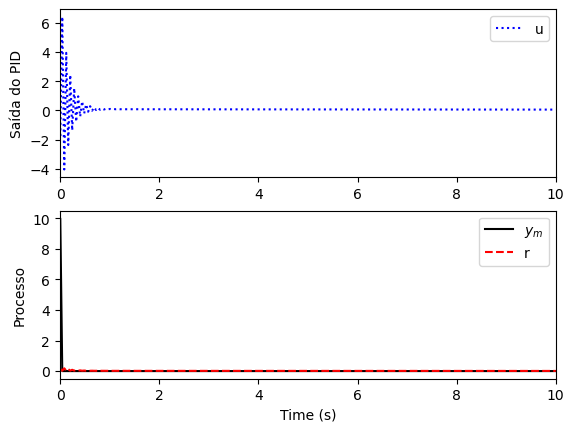
\includegraphics[scale=.49]{pid.png}
     \label{fig:pid2024}
\end{figure}
\vspace*{-0.8cm}
{\raggedright \fonte{Autor.}}

Pela Figura \ref{fig:pid2024}, observe que a saída \(u\) assume valores contínuos, mas o ambiente \textit{Cart Pole} utilizado é discreto (1 para força à direita e 0 para força à esquerda). Para resolver esse problema, foi implementada a seguinte estratégia: se \(u > 0\), é aplicada uma força à direita; caso contrário, é aplicada uma força à esquerda.

\section{\textit{Cart Pole}: Controle Preditivo Generalizado Aplicado}
\label{sec:GPCcartpole}    

Na presente seção, contém o processo para derivar a trajetória de referência, a função custo e obter o modelo ARX. Os princípios delineados na Seção \ref{sec:CPG} foram aplicados em um algoritmo para a realização dessas tarefas.

\subsection{Controle Preditivo Generalizado: Formulação para o \textit{Cart Pole}}
\label{subsec:GPCfor}  

A trajetória de referência ($w$) representa o comportamento do sinal desejado para a saída futura, sendo o primeiro passo na aplicação do controle preditivo generalizado (GPC). No caso do pêndulo invertido, ela será 0, pois a ideia é manter o pêndulo estável, o que implica em minimizar o $\theta$, de maneira:

\begin{equation}
    w = [0, 0, 0, \cdots, n_{etapas}],
    \label{eq:traref}
\end{equation}

\noindent considerando que $n_{etapas}$ representa o número total de etapas.

O próximo passo consiste em estabelecer uma função de custo, considerando as recompensas do ambiente \textit{Cart Pole}. Nesse contexto, uma recompensa é atribuída por cada passo dado, abrangendo inclusive a etapa de encerramento, uma vez que o objetivo é manter o poste ereto pelo maior tempo possível. O limite estabelecido para as recompensas é de 500\cite{gymcartpole}. Logo, o esforço de controle não será penalizado, apenas o erro em relação à predição da saída e à referência:

\begin{equation}
    J(k) =\sqrt{(\sum_{j=d}^{h_p} [\hat{y}(j+k|k) - w(j+k)])^2}.
    \label{eq:FO}
\end{equation}

A função de custo utilizada enfatiza a capacidade do parâmetro $\theta$ de mudar de sinal, possibilitando sua proximidade ao limiar de 0 radianos.

No entanto, ainda é necessário identificar um modelo capaz de prever a saída ($\hat{y}$) em função de $\Delta u$, seguindo a metodologia do GPC. Nesse contexto, a saída é representada por 1 para movimento à direita e -1 para movimento à esquerda, a fim de manter consistência com a codificação utilizada na FT.  Isso resulta em $\Delta u$ assumindo três valores inteiros, o que se justifica por:

\begin{equation}
    \begin{matrix}
        u_{k-1} = 1 \text{ e } u_{k} = -1 \Rightarrow \Delta u = -2 \\
        u_{k-1} = 1 \text{ e } u_{k} = 1 \Rightarrow \Delta u = 0\\
        u_{k-1} = -1 \text{ e } u_{k} = -1 \Rightarrow \Delta u = 0\\
        u_{k-1} = -1 \text{ e } u_{k} = 1 \Rightarrow \Delta u = 2 \\
    \end{matrix}.
\end{equation}

A definição do problema de otimização é a seguinte:

\begin{equation}
    \begin{matrix}
        \textbf{Minimizar} & J(k) =\sqrt{(\sum_{j=d}^{h_p} [\hat{y}(j+k|k) - w(j+k)])^2}\\
        \text{sujeto a:} &  \Delta u = \{-2, 0, 2\}
    \end{matrix}.
\end{equation}

Para minimizar essa função custo, emprega-se o Método de Pesquisa em Grade, o qual é detalhado na Seção \ref{sec:MPG}. Esse método consiste em uma abordagem sistemática que varre diferentes combinações de parâmetros dentro de um intervalo predefinido (as combinações da entrada), buscando encontrar o conjunto ótimo que resulta na minimização da função custo.

\subsection{Estimação do Modelo ARX}
\label{subsec:GPCfor}  

Nesta seção há o processo de identificação do modelo ARX do sistema, utilizando um sinal PRBS (do inglês, \textit{Pseudo-Random Binary Sequence}) para excitar o \textit{Cart Pole}. O PRBS \cite{aguirre2004} assume apenas dois valores possíveis, $+V$ e $-V$. Além de ser fácil de implementar, é replicável, o que o torna bastante popular na identificação de sistemas. 

O menor intervalo no qual o nível do sinal é mantido é denominado $T_b$. Seu período pode ser determinado por $T = NT_b$, sendo $N$ um número ímpar, de modo que $T_b = T_s$. Um resultado heurístico para a escolha de $T_b$ é: $\frac{\tau_{\text{min}}}{10} \leq T_b \leq \frac{\tau_{\text{min}}}{3}$, onde $\tau_{\text{min}}$ representa a menor constante de tempo de interesse, sugerida por Nelles (2001) \cite{nelles}, que, para sistemas lineares, $T_b$ seja escolhido próximo ao valor do intervalo de amostragem. Para sistemas não lineares, por outro lado, recomenda-se que $T_b$ seja aproximadamente igual a $\tau_{max}$, onde $\tau_{max}$ é a constante de tempo do sistema.

Trabalhando com um modelo ARX, considera-se o tempo de amostragem $T_b$. Assim, obtém-se a saída devido ao PRBS conforme mostrado na Figura \ref{fig:PRBSa}.

\begin{figure}[H]
     \centering
     \vspace*{-.2cm}
     \caption{Aplicando o PRBS.}
     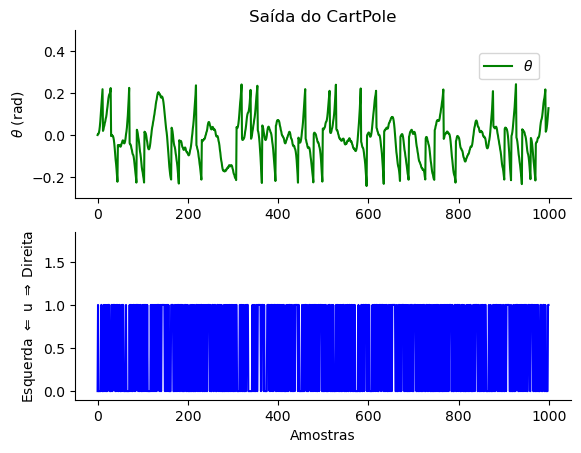
\includegraphics[scale=0.575]{teste.png}
     \label{fig:PRBSa}
\end{figure}
\vspace*{-0.7cm}
{\raggedright \fonte{Autor.}}

É importante observar que o ambiente \textit{Cart Pole} reinicia automaticamente sempre que atinge um desvio de aproximadamente $\pm 12^\circ$ (equivalente a $\pm 0,209$ radianos). Essa característica representa um desafio, pois resulta em episódios muito curtos, dificultando a estimativa do modelo ARX. Inicialmente, uma abordagem para solucionar esse problema poderia envolver a redução do intervalo de tempo $T_b$. Isso implicaria em uma diminuição no tempo de amostragem do sistema, permitindo que as ações sejam executadas em períodos mais curtos e, assim, estendendo a duração dos episódios.

No entanto, é crucial observar que essa abordagem não é viável no contexto do ambiente \textit{Cart Pole} no Gymnasium. Isso se deve ao fato de que a taxa de amostragem no ambiente \textit{Cart Pole} não é diretamente ajustável. O ambiente \textit{Cart Pole} foi projetado para simular a física real associada ao problema de um pêndulo invertido sobre um carro, e a taxa de amostragem é intrínseca a essa simulação. Portanto, modificar diretamente a taxa de amostragem do ambiente não é uma opção disponível. Esse aspecto limita a capacidade de ajuste do tempo de amostragem para atender às necessidades específicas do modelo ARX no contexto do problema \textit{Cart Pole}.

Para enfrentar essa tarefa complexa, foram realizadas 2 milhões de iterações no ambiente de simulação. Dentre essas iterações, o episódio mais longo, com o maior número de passos ou amostras, foi cuidadosamente selecionado para a estimativa do modelo ARX. Este episódio em particular se estende por 183 amostras, fornecendo assim uma base robusta e abrangente para a análise e modelagem do sistema. A escolha deste episódio mais extenso mostrado na Figura \ref{fig:PRBSz} assegura que tenhamos dados significativos o suficiente para capturar as nuances e complexidades do sistema, permitindo uma estimativa precisa do modelo ARX.

\begin{figure}[H]
     \centering
     \vspace*{-.2cm}
     \caption{Maior episódio.}
     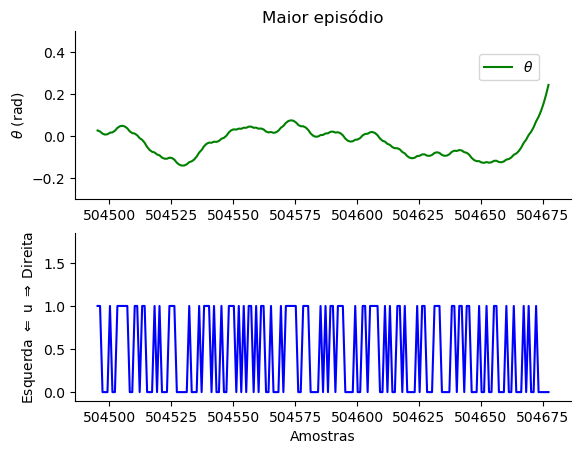
\includegraphics[scale=0.575]{mep.png}
     \label{fig:PRBSz}
\end{figure}
\vspace*{-0.7cm}
{\raggedright \fonte{Autor.}}

Serão utilizados 158 amostras para o treinamento do modelo, sendo as 25 restantes empregadas para validação. O modelo ARX encontrado pelo SysIdentPy, foi:

\begin{equation}
    y(k) = 2\cdot y(k-1)- 0,99367\cdot y(k-2)  - 0,00583\cdot u(k-1),
    \label{eq:28}
\end{equation}

\noindent sendo $RMSE = 0,0057$.

Para lidar com a instabilidade do \textit{Cart Pole}, adotou-se um horizonte de controle igual de predição ($H_p=H_c$), ajustando $H_c$ com foco na eficiência do controle e tempo de execução, considere o tempo de execução ($t$) segundos para ($H_c=2$), conforme apresentado na Tabela \ref{tab:HCcartpole}.
 
\begin{table}[H]
	\centering
	\vspace*{-.2cm}
	\caption{Horizonte de Controle em relação ao Tempo.}
	\begin{tabular}{|c|c|c|c|c|c|c|c|}
	\hline
           Horizonte de Conrole $(H_c)$ & $2$ & $3$ & $4$ & $5$ & $6$ & $7$ \\
            \hline
            Tempo de Execução $[s]$ & $t$ & $1,071$ & $1,218t$ & $1,8164t$ & $3,58t$ & $9,18t$\\ 
            \hline
	\end{tabular}  
    \label{tab:HCcartpole}                 % Nome da tabela para referência cruzada
\end{table}
\vspace*{-0.7cm}
{\raggedright \fonte{Autor.}}

A escolha do horizonte de controle de 4 foi baseada na análise de que, apesar do aumento modesto no tempo de execução ao passar de 3 para 4, a transição de 4 para 5 representa um intervalo mais significativo. A lógica subjacente é buscar o maior horizonte de controle viável, minimizando simultaneamente o tempo de execução.

\section{\textit{Lunar Lander}: Implementação e Sintonia do Controlador PD}
\label{sec:pidLunarLander} 

Nesta seção, é abordada a implementação do controlador PID passo a passo, com o objetivo de controlar a \textit{Lunar Lander}. No entanto, se trata de uma abordagem um pouco mais empírica em comparação com o \textit{Cart Pole}.

\subsection{\textit{Lunar Lander}: Aplicando o controle PD}
\label{sec:pidLunarLanderEC} 

O controlador PD foi retirado do repositório Lunar Lander\_OpenAIGym \cite{llpid} com algumas modificações. A ideia de modelar o sistema por meio de um modelo caixa branca não foi bem-sucedida, uma vez que se trata de um sistema MIMO, o que eleva o grau de complexidade. Seria necessária uma função de transferência para cada entrada e saída, tornando complicada a determinação dos parâmetros intrínsecos ao sistema. Assim, este repositório apresenta uma abordagem mais empírica, semelhante ao que ocorre no meio industrial, onde o PID é amplamente utilizado.

A plataforma de aterrissagem permanece fixa nas coordenadas (0,0), sendo permitido a possibilidade de pouso fora da área designada. Além disso, é importante ressaltar que não há restrições quanto ao combustível, sendo considerado infinito para a execução da tarefa.

O primeiro passo é determinar as variáveis de processo a serem controladas, sendo os \textit{boosters} do motor principal e secundário, usados respectivamente para controlar a altitude e o ângulo e/ou posição horizontal da nave.


A sonda ajusta-se com base nos sensores para minimizar erros ao longo do tempo, utilizando controle proporcional-derivativo (PD). Altitude, ângulo e velocidades são conhecidos em cada etapa. O erro é calculado como a diferença entre os \textit{setpoints} e as medições atuais, permitindo controle proporcional. As velocidades são usadas para o controle derivativo. Para a implementação do PD, os pontos de ajuste (\textit{setpoints}) serão definidos, conforme ilustrado na Figura \ref{fig:aa}.

\begin{figure}[H]
    \definecolor{lightred}{RGB}{156,207,237} 
    \definecolor{igreen}{RGB}{0, 143, 0}
    \definecolor{rpurple}{RGB}{156, 112, 214}
    \centering
    \hspace*{-.2cm}
    \vspace*{-.3cm}
    \caption{\textit{Setpoints} para o controle PD.}
    \begin{tikzpicture}
    % Corpo da sonda
        \draw (0,-3)rectangle (8,1);
        \draw[fill=white] (0, -3) rectangle (8,-3.1);
        \draw[fill=white] (2.5, -3) rectangle (2.6,-2.25);
        \draw[fill=yellow] (2.6,-2.5) -- (2.6,-2.25) -- (3,-2.375) -- cycle;
        \draw[fill=white] (5.25, -3) rectangle (5.35,-2.25);
        \draw[fill=yellow] (5.35,-2.5) -- (5.35,-2.25) -- (5.75,-2.375) -- cycle;
        \draw[color=black, line width=2pt] (4,-3) -- (0,1) ;
        \draw[color=black, line width=2pt] (4,-3) -- (8,1) ;
        \node at (1.3, -1.5){$|x|>y$};
        \node at (1.3, -1.9){\small \color{red}{Elevar altura}};
        \node at (6.7 , -1.5){$|x|>y$};
        \node at (6.7, -1.9){\small \color{red}{Elevar altura}};
        \node at (4, -1.5){$|x|<y$};
        \node at (4, -1.1){\small \color{igreen}{Reduzir
        altura}};
        \draw[->, color=blue, line width=1.1pt] (4, -3) -- (4,-2) node[right] {$y$};
        \draw[->, color=blue, line width=1.1pt] (3.99, -3) -- (5,-3) node[above] {$x$};
        \node at (4, 1.25){Altura};
        \node at (4, 0.6){$|x|: $ É o \textit{setpoint}};
        %Figura 2
        \draw[fill= green!20] (8.25,1)--(12.25,-3)--(16.25,1);
        \draw (8.25,-3)rectangle (16.25,1);
        \draw[fill=white] (8.25, -3) rectangle (16.25,-3.1);
        \draw[color=black, line width=2pt] (12.25,-3) -- (8.25,1) ;
        \draw[color=black, line width=2pt] (12.25,-3) -- (16.25,1);
        \draw[fill=rpurple, color=rpurple,cm={cos(45) ,-sin(45) ,sin(45) ,cos(45) ,(3 cm,7.375 cm)}] (9.75,-1)--(10.75,-1)--(10.6,-.5)--(9.9,-.5)-- (9.75,-1);
        \draw(9.7,-0.4)[->]--(11.25, -0.4) node[above] {\small $x$}[->]--(12.25, -0.4); 
        \draw[dashed] (12.25,-3) -- (12.25,-.35);
        \draw[->, color=red, line width=.5pt] (9.685, -0.4) -- (10.2,-0.4) node[above] {\small $x$};
        \draw
        (10.05,-0.05) coordinate (a) node[right] {}
        -- (9.7,-0.395) coordinate (b) node[left] {}
        -- (9.7,0.1) coordinate (c) node[above right] {}
        pic["\small $\theta$",draw=orange, <->, angle eccentricity=1.35, angle radius=.5cm]
        {angle=a--b--c};
        \draw[->, color=red, line width=.5pt] (9.7, -0.4) -- (9.7,0.1) node[above] {\small $y$};
        \draw[->, color=red, line width=.5pt] (9.7, -0.4) -- (10.05,-0.05) node[above right] {\small $N$};
        \draw[fill=blue] (9.7,-0.4) circle (.05); 
        \node at (12.25, 1.25){Ângulo};
        \node at (9.92, -2.7){\small $\theta$: Ângulo da sonda};
        \draw[fill=blue] (8.5,-2.3) circle (.05) node [right]{\small : Centro de massa}; 
        \draw[->, color=blue, line width=1.1pt] (12.25, -3) -- (12.25,-2) node[right] {$y$};
        \draw[->, color=blue, line width=1.1pt] (12.24, -3) -- (13.25,-3) node[above] {$x$};
        \node at (12.65, 0.6){$\frac{\pi}{4}(x+v_x): $ É o \textit{setpoint}};
        \node at (14.65, -2.4){\small $x+v_x = x + \frac{d x(t)}{dt}$};
        % Adicione outros detalhes conforme necessário
    \end{tikzpicture}
    \label{fig:aa}
\end{figure}
\vspace*{-1cm}
{\raggedright \fonte{Autor.}}

O primeiro \textit{setpoint} considerado é a altura, com a posição $x$ como \textit{setpoint}, conforme a Figura \ref{fig:aa}. Se a sonda estiver dentro do triângulo, deve descer, caso contrário, deve subir. Isso define o termo proporcional. Para o termo derivativo, utiliza-se a velocidade linear em $y$:

\begin{equation}
    y_{PD} = k_{p2}\cdot (|x|-y)+k_{d2}\cdot v_y.
    \label{eq:ypd}
\end{equation}


É crucial manter uma inclinação constante da nave em direção ao seu objetivo, pois isso determina a direção do impulso do propulsor principal. Para implementar essa abordagem, utiliza-se o \textit{setpoint} $x + v_x$, onde $v_x$ é a taxa de variação em $x$, entendendo essa expressão como $x_{t+1}$ para minimizar $\theta$. Quando a sonda está nas bordas extremas do triângulo, ela deve se inclinar $ 45^\circ$ em direção a plataforma, com essa inclinação diminuindo à medida que a sonda se aproxima do alvo (0,0), de acordo com o \textit{setpoint} $x_{t+1}$. O controle proporcional é aplicado, onde a posição $x$ diminui à medida que a sonda se aproxima do alvo, enquanto o termo derivativo utiliza a velocidade angular:

\begin{equation}
    \theta_{PD} = k_{p2}\cdot \bigg{[} \frac{\pi}{4}\cdot (x+v_x)-\theta\bigg{]}+k_{d2}\cdot v_{\theta}.
    \label{eq:tpd}
\end{equation}

Todos os elementos essenciais foram identificados, exceto pelos valores apropriados dos quatro parâmetros $k_{p1}$, $k_{d1}$, $k_{p2}$ e $k_{d2}$. Para determinar esses pesos, foi adotada a técnica de Otimização por Subida de Encosta. Ao que tudo indica, diferentemente do que é feito no repositório LunarLander\_OpenAIGym \cite{llpid}, onde $k_p$ e $k_d$ são iguais no PD referente ao ângulo e à altura, o que leva a crer que foi sintonizado manualmente. Essa metodologia inicia com a premissa de que todos os parâmetros são inicialmente nulos (sem controle). Após cada tentativa de aterrissagem da sonda e avaliação da pontuação, os parâmetros são ajustados com pequenas variações aleatórias. Se a pontuação da sonda melhorar, os novos valores são mantidos e o processo é repetido. Caso contrário, os novos valores são descartados e tenta-se adicionar ruído aleatório novamente. Os valores encontrados foram: $k_{p1} = 9,0565$, $k_{d1} = -9,9488$, $k_{p2} = 11,9271$ e $k_{d2} = -5,0963$. 

\section{\textit{Lunar Lander}: Controle Preditivo Generalizado Aplicado}
\label{sec:GPCfor}    

Nesta seção, detalha-se o processo de obtenção das trajetórias de referência e da função custo, bem como a derivação do modelo ARX. A metodologia descrita na Seção \ref{sec:CPG} foi incorporada em um algoritmo.

\subsection{Controle Preditivo Generalizado: Formulação para o \textit{Lunar Lander}}
\label{subsec:GPCtr}   

As trajetórias de referência ($w$) do \textit{Lunar Lander} são um pouco mais complexa, na qual serão adotadas algumas estratégias. 

Sabe-se que o ambiente no qual a sonda interage é traduzido por meio de um plano cartesiano. Essa abordagem permite conhecer valores como posição e direção, aspectos de suma importância na navegação da sonda.

Com intuito de implementar o GPC, foi empregado uma matriz rotação para rotacionar o plano cartesiano em $45^\circ$ (o motivo será explicado adiante), por ser bidimensional, tem-se:

\begin{equation}
	\begin{bmatrix}
		p_x\\
		p_y\\
	\end{bmatrix}
    = 
    \begin{bmatrix}
        cos \phi & sen\phi\\
        -sen \phi & cos \phi\\
    \end{bmatrix}
    \begin{bmatrix}
        x\\
        y\\
    \end{bmatrix}.
\end{equation}

Se considerar $\phi = 45^\circ$ e respectivos valores fornecidos pelo ambiente de observação:

\begin{equation}
\begin{split}
    p_x = x\cdot cos\:45^\circ +  y\cdot sen\:45^\circ\\
    p_y = -x\cdot sen\:45^\circ +  y\cdot cos\:45^\circ\\
\end{split}.
\end{equation}

A ideia é rotocionar o plano cartesiano como ilustrado na Figura \ref{fig:pc45}.

\begin{figure}[H]
    \centering
    \vspace*{-.2cm}
    \caption{Plano cartesiano do \textit{Lunar Lander},}
    \begin{tikzpicture}
        % Figure 2
        \draw
          (12.25,0) coordinate (a) node[right] {}
        -- (12.25,-3) coordinate (b) node[left] {}
        -- (10.12867,-0.87867) coordinate (c) node[above right] {};
        \draw (8.25,-3) rectangle (16.25,1);
        \draw[fill=white] (8.25, -3) rectangle (16.25,-3.1);
        \draw[fill=white] (10.75, -3) rectangle (10.85,-2.25);
        \draw[fill=yellow] (10.85,-2.5) -- (10.85,-2.25) -- (11.25,-2.375) -- cycle;
        \draw[fill=white] (13.5, -3) rectangle (13.6,-2.25);
        \draw[fill=yellow] (13.6,-2.5) -- (13.6,-2.25) -- (14,-2.375) -- cycle;
        \draw[->, color=blue, line width=1.1pt] (12.25,-3) -- (12.25,1) node[below right] {$y$};
        \draw[->, color=blue, line width=1.1pt] (12.25,-3) -- (16.25,-3) node[above left] {$x$};
        %\node[left] at (16.15,-2.75) {$x$};
        \draw[->, line width=1.1pt] (12.25,-3) -- (9.45,-0.2)node[above] {$p_y$};
        \draw pic["\small $\phi=45^\circ$",draw=orange, <->, angle eccentricity=1.35, angle radius=1.5cm]
        {angle=a--b--c};
        \draw[->, line width=1.1pt] (12.25,-3) -- (15.05,-0.2)node[above] {$p_x$};
        % Adicione outros detalhes conforme necessário
    \end{tikzpicture}
    \label{fig:pc45}
\end{figure}
\vspace*{-0.5cm}
{\raggedright \fonte{Autor.}}

Com o plano cartesiano rotacionado, é possível estimar três trajetórias de referência. A primeira, em ciano, é definida por $p_x=p_y$. Similarmente ao \textit{Cart Pole}, o ângulo $\theta$ do \textit{Lunar Lander} deve estar próximo de zero, representando a segunda trajetória de referência. O próximo passo envolve determinar a terceira trajetória de referência para a velocidade linear em $p_y$, expressa por $v_{y} = -0,725\cdot p_y - 0,125$. Esta ideia será ilustrada na Figura \ref{fig:llset}.

\begin{figure}[H]
    \definecolor{rpurple}{RGB}{156, 112, 214}
    \centering
    \vspace*{-.25cm}
    \caption{\textit{Setpoints} para o GPC,}
    \begin{tikzpicture}
        \definecolor{darkgreen}{RGB}{0,100,0} 
        \draw (7,-3) rectangle (17.5,1);
        \draw[fill=white] (7, -3) rectangle (17.5,-3.1);
        \draw[fill=white] (10.75, -3) rectangle (10.85,-2.25);
        \draw[fill=yellow] (10.85,-2.5) -- (10.85,-2.25) -- (11.25,-2.375) -- cycle;
        \draw[fill=white] (13.5, -3) rectangle (13.6,-2.25);
        \draw[fill=yellow] (13.6,-2.5) -- (13.6,-2.25) -- (14,-2.375) -- cycle;
        \draw[->, line width=1.1pt] (12.25,-3) -- (9.45,-0.2)node[left] {\small $p_y$};
        \draw[->, line width=1.1pt] (12.25,-3) -- (15.05,-0.2)node[right] {\small $p_x$};
        \draw[dashed, line width=1.1pt, color=darkgreen] (12.25,-3) -- (12.25,0.45) node[above]{\footnotesize \textit{Setpoint}: $p_x=p_y$};
        \draw[fill=rpurple, color=rpurple] (11.75,-1)--(12.75,-1)--(12.6,-.5)--(11.9,-.5)-- (11.75,-1);
        \draw[->,line width=1.1pt,  blue](12.25,-.75)--(12.25,-1.25);
        \draw[fill=blue] (12.25,-.75) circle (.05); 
        \node at (12.4,-.5)[above right,  line width=1.1pt, color=violet]{\footnotesize \textit{Setpoint}: $\theta =0$};
        \node at (6.935,-.15)[above right,color=blue]{\footnotesize \textit{Setpoint}: $v_y = -0,725\cdot p_y - 0,125$};
        % Adicione outros detalhes conforme necessário
    \end{tikzpicture}
    \label{fig:llset}
\end{figure}
\vspace*{-0.5cm}
{\raggedright \fonte{Autor.}}

Para estimar o modelo ARX e facilitar a compreensão, os propulsores auxiliares de orientação direita e esquerda foram considerados como um só ($u_2$), assumindo 1 para direita e -1 para esquerda, com 0 representando a condição desligada. Para o propulsor principal ($u_1$), 1 indica o acionamento e 0 representa que está desligado.

Em relação ao incremento de controle ($\Delta u$), uma metodologia alternativa está sendo considerada para o ambiente \textit{Lunar Lander}. Enquanto o MPC tradicionalmente penaliza o $\Delta u$ com base em sua magnitude, neste contexto lunar específico, a penalização varia com os propulsores: auxiliares têm penalização de 0,03, o principal de 0,3 e nenhum acionamento não é penalizado. Dessa forma, a proposta é focar no controle absoluto $u$ em vez do incremento $\Delta u$. Quando o horizonte de controle ($H_c$) é menor que o de previsão ($H_p$), $u$ é mantido em 0, permitindo respostas que maximizam a recompensa do ambiente.

Conforme mencionado anteriormente, a metodologia de aplicação do modelo define a função de custo conforme a Equação \ref{eq:custogpc}:

\begin{equation}
\label{eq:custogpc}
\begin{matrix}
    J(k) = \sum_{j=d}^{h_p}[\{\alpha\cdot (\hat{p}_x(j+k|k) - \hat{p}_y(j+k|k) )-\beta \cdot \hat{\theta}(j+k|k)\\
            +\delta \cdot  (\hat{v}_y(j+k|k)-0,725\cdot\hat{p}_y(j+k|k)-0,125)\}^2]^\frac{1}{2}\\
\end{matrix},
\end{equation}

\begin{equation*}
\begin{matrix}
  \text{sujeito a:} &  \\
  	Propulsor = & 
  	\left\{
  	\begin{matrix}
  	0  & 0 & 1 & 0 \\
   -1  & 0 & 0 & 1
	\end{matrix}  	
	\right\} 
	\begin{matrix}
  	u_1 \Rightarrow\text{Propulsor principal}\\
    u_2 \Rightarrow\text{Propulsor auxiliar}
	\end{matrix}
\end{matrix}.
\end{equation*}

As entradas devem ser intercaladas ou completamente desligadas. Em outras palavras, se uma estiver ativa, a outra deve permanecer desligada, ou ambas devem estar desligadas simultaneamente. O horizonte de controle foi definido como igual a 2 ($H_c=2$) e o horizonte de predição como 4 ($H_p=4$). Esses valores foram definidos experimentalmente e, apesar de serem pequenos, apresentaram uma boa resposta com um excelente tempo de execução.

\subsection{Estimação do Modelo ARX}
\label{subsec:GPCforLL}  

Nesse processo, optou-se por empregar uma entrada aleatória, com o objetivo de obter um modelo para as coordenadas $p_x$ e $p_y$, $\theta$ e $v_y$ (velocidade linear em y). Durante a obtenção do modelo, observou-se uma correlação de cada uma das saídas com uma entrada específica, conforme evidenciado pela Tabela \ref{tab:intlla}.

\begin{table}[H]
	\centering
	\vspace*{-.2cm}
	\caption{Relação entre entradas e saídas.}
	\begin{tabular}{|c|c|c|c|c|}
			\hline
             Saída & $p_x$ & $\theta$ & $p_y$ & $v_y$ \\
            \hline
            Entrada & $u_2$ & $u_2$ & $u_1$ & $u_1$\\ 
            \hline
	\end{tabular}  
    \label{tab:intlla}                 % Nome da tabela para referência cruzada
\end{table}
\vspace*{-0.7cm}
{\raggedright \fonte{Autor.}}

Dessa forma, por meio da metodologia começou-se a investigar várias alternativas para cada entrada. A cada iteração, um valor era selecionado aleatoriamente dentre as opções disponíveis. Para $u_1$, o intervalo considerado foi [0, 2] do ambiente e [0, 1] para a identificação, enquanto $u_2$ apresentava três possíveis respostas [0, 1, 3] e [0, 1, -1] para a identificação.

 Novamente, foi usado o SysIdentPy para estimar os modelos ARX para os itens já mencionados:

\begin{equation}
\begin{matrix}
    p_x(k) = 1,9986\cdot p_x(k-1) -0,9986 \cdot p_x(k-2)\\
    -7,3642\cdot 10^{-5}\cdot u_2(k-1) -4,7979\cdot 10^{-4}\Rightarrow RMSE=0,0009,
\end{matrix} 
\end{equation}

\begin{equation}
\begin{matrix}
    p_y(k) = 1,9928\cdot p_y(k-1) - 0,99279\cdot p_y(k-2)\\
    +8,1745\cdot 10^{-5}\cdot u_1(k-1) -3,9457\cdot 10^{-4}\Rightarrow RMSE=0,0355,
\end{matrix} 
\end{equation}

\begin{equation}
\begin{matrix}
    \theta(k) = -1,9891\cdot \theta(k-1) +0,989\cdot \theta(k-2)\\
    +1,7201\cdot 10^{-4}\cdot u_2(k-1)\Rightarrow RMSE=0,0007,
\end{matrix} 
\end{equation}

\begin{equation}
\begin{matrix}
    v_y(k) = 1,2503\cdot v_y(k-1) - 0,25137\cdot v_y(k-2)\\
    -1,3791\cdot 10^{-2}\cdot u_1(k-1)+2,3644\cdot 10^{-3}\Rightarrow RMSE=0,0549.
\end{matrix} 
\end{equation}

Mesmo com o uso de apenas 70 amostras para a identificação do modelo, o SysIdentPy demonstrou um desempenho notável ao capturar um modelo de alta qualidade para o \textit{Lunar Lander}, sendo validado por 15 amostras. Esse desempenho ressalta a eficácia e a robustez do pacote SysIdentPy, que conseguiu extrair informações precisas o suficiente das amostras disponíveis para formar um modelo que adequadamente representa a complexa dinâmica do \textit{Lunar Lander}.

\subsection{Determinação dos Pesos da Função Custo}
\label{subsec:GPCpesos}  

Inicialmente, a estimação dos pesos foi feita por tentativa e erro, onde foram identificados alguns pontos importantes posteriormente utilizados. O principal foi a separação do ambiente lunar em dois estágios. O primeiro estágio consiste em verificar se a velocidade da sonda é inferior à trajetória de referência. Nesse caso, o peso $\delta$ na Equação \ref{eq:custogpc}, sendo zero, ajuda o modelo a não tomar decisões equivocadas, como inclinar em um ângulo $\theta$ grande e utilizar os motores auxiliares para acelerar e alcançar a referência. Dessa maneira, a sintonização manual se tornou mais tranquila, onde no primeiro estágio o algoritmo monitora apenas com os \textit{setpoints} de posição e inclinação angular. No segundo estágio, a velocidade linear em $y$ passa a fazer parte dos \textit{setpoints}.

Depois de muitas tentativas, o GPC apresentou resultados semelhantes ao PD do repositório LunarLander\_OpenAIGym. No entanto, ao adotar um algoritmo de Subida de Encosta para estimar os parâmetros proporcionais e derivativos do PD deste trabalho, houve uma melhoria significativa no desempenho do PD. Assim, um ajuste manual do GPC para se equiparar ao PD tornou-se complicado. A proposta consistiu em aplicar o algoritmo de Subida de Encosta para estimar os pesos do segundo estágio ($\alpha_2$, $\beta_2$, e $\delta_2$), enquanto os pesos do primeiro estágio foram previamente definidos manualmente como $\alpha=\beta=1$ e $\delta=0$, mantidos devido ao seu desempenho satisfatório. Os pesos encontrados se encontram na Figura \ref{fig:setp12}.

\begin{figure}[H]
    \definecolor{rpurple}{RGB}{156, 112, 214}
    \centering
    \vspace*{-.2cm}
    \caption{Pesos da Função de Custo para o \textit{Lunar Lander}.}
    \begin{tikzpicture}
        \draw[fill=green!20] (8.25,0) rectangle (16.25,1);
        \draw[fill=cyan!25] (8.25,0) rectangle (16.25,-3);
        \draw (8.25,-3) rectangle (16.25,1);
        \draw[fill=green!20] (8.25,0) rectangle (16.25,1);
        \draw[fill=white] (8.25, -3) rectangle (16.25,-3.1);
        \draw[fill=white] (10.75, -3) rectangle (10.85,-2.25);
        \draw[fill=yellow] (10.85,-2.5) -- (10.85,-2.25) -- (11.25,-2.375) -- cycle;
        \draw[fill=white] (13.5, -3) rectangle (13.6,-2.25);
        \draw[fill=yellow] (13.6,-2.5) -- (13.6,-2.25) -- (14,-2.375) -- cycle;
        \draw[color=red, line width=1.5pt] (8.25,0) -- (16.25,0);
        \node at (12.25,.53)[above]{\scriptsize $\beta_1 = 1$};
        \node at (12.25,.23)[above]{\scriptsize $\alpha_1 = 1$};
        \node at (12.25,-.07)[above]{\scriptsize $\delta_1 = 0$};
        \node at (12.25,-1.6)[above]{\scriptsize $\beta_2 = 23,1039$};
        \node at (12.25,-1.9)[above]{\scriptsize $\alpha_2 = 3,6923$};
        \node at (12.25,-2.2)[above]{\scriptsize $\delta_2 = 58,5223$};
        \node at (8.25,.5)[right]{\scriptsize $1^\circ$ Estágio};
        \node at (8.25,-1.5)[right]{\scriptsize $2^\circ$ Estágio};
        \draw[->, color=red,  line width=1.5pt](12.25,0)--(12.25,-.25) node[below]{\scriptsize $\hat{y}_v[0]=-0,725\hat{p}_y[0]-0,125$};;
        % Adicione outros detalhes conforme necessário
    \end{tikzpicture}
    \label{fig:setp12}
\end{figure}
\vspace*{-0.7cm}
{\raggedright \fonte{Autor.}}

Os pesos ($\alpha_2$, $\beta_2$ e $\delta_2$) derivados pelo algoritmo de subida de Encosta resultaram em uma notável melhoria no desempenho do Controle Preditivo Generalizado (GPC), em comparação com os ajustes manuais realizados por tentativa e erro. Essa otimização automática permitiu uma sintonia mais precisa e eficiente dos parâmetros do controlador, levando a um funcionamento mais eficaz do sistema de controle.\\

%%%%%%%%%%%%%%%%%%%%%%%%%%%%%% RESULTADOS (OBRIGATÓRIO) %%%%%%%%%%%%%%%%%%%%%%%%%%%%%%
		
{\let\clearpage\relax\par \chapter{RESULTADOS}}
\label{ch:resultados}                       % Nome do capítulo para referência cruzada

\section{\textit{Cart Pole}}

A seguir, encontra-se um GIF que ilustra o funcionamento do Controle PID e GPC:

\begin{figure}[H]
  \begin{minipage}{0.5\textwidth}
    \centering
    \caption{PID: \textit{Cart Pole} GIF.}
    \animategraphics[width=.875\textwidth, loop, autoplay]{30}%frame rate
    {ctpid.png/4e94350248dc4151dd0ed2d1e64d0993Iavq0D3A7278MZjZ-}%path to figures
    {0}%start index
    {499}%end index
    \label{fig:GPC1}
  \end{minipage}
  \begin{minipage}{0.5\textwidth}
    \centering
    \caption{GPC: \textit{Cart Pole} GIF.}
    \animategraphics[width=.875\textwidth, loop, autoplay]{30}%frame rate
    {ctmpc.png/242c88173bef4e85e035f2a79b9761b3fZwHX7Am1w0pwG0a-}%path to figures
    {0}%start index
    {499}%end index
    \label{fig:PID1}
  \end{minipage}
\end{figure}
\vspace*{-.7cm}
{\raggedright \fonte{Autor.}}

Para facilitar a compreensão, é útil representar o compotameto do \textit{Cart Pole} de maneira gráfica:

\begin{figure}[H]
  \begin{minipage}{0.5\textwidth}
    \centering
     \caption{PID: \textit{Cart Pole}.}
     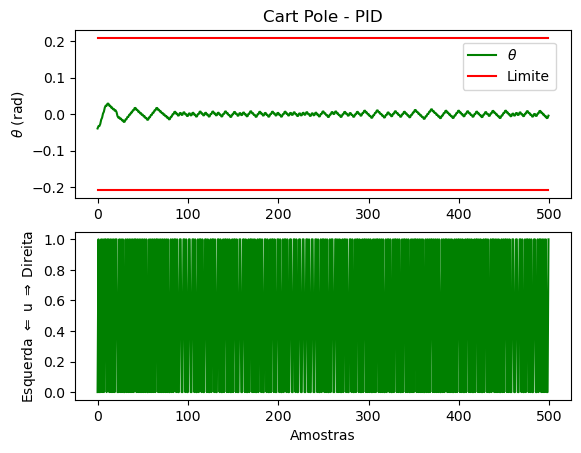
\includegraphics[scale=0.47]{ctpidio.png}
    \label{fig:imagem1}
  \end{minipage}
  \begin{minipage}{0.5\textwidth}
    \centering
     \caption{GPC: \textit{Cart Pole}.}
     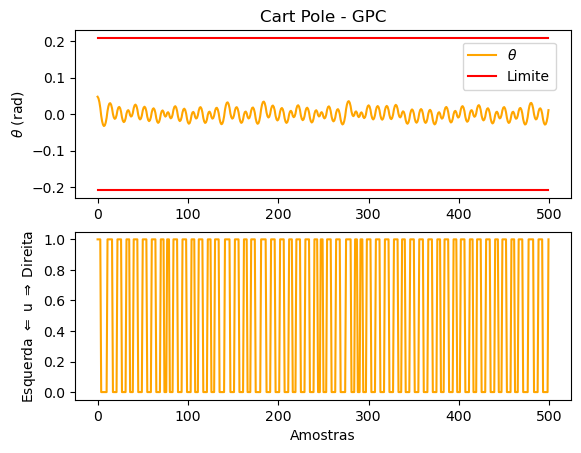
\includegraphics[scale=0.47]{ctgpcio.png}
    \label{fig:imagem2}
  \end{minipage}
\end{figure}
\vspace*{-.9cm}
{\raggedright \fonte{Autor.}}

Ambas as estratégias de controle (GPC e PID) demonstraram ser capazes de controlar o sistema, entretanto, o PID foi mais eficaz em manter o \textit{Cart Pole} mais próximo a referência ($\theta=0$):

\begin{table}[H]
	\centering
	\vspace*{-.2cm}
	\caption{PID x CPC - \textit{Cart Pole}.}
	\begin{tabular}{|c|c|c|c|c|}
			\hline
             Controle & $\bar{\theta}$ & $\theta_{max}$ & Etapas & Tempo de Execução $[s]$\\
            \hline
            PID & $1,1053\cdot 10^{-5}$ & $4,6395\cdot 10^{-2}$ & 5000 & $9,0421$\\
            \hline
            GPC & $-9,7546\cdot 10^{-5}$ & $7,3337\cdot 10^{-2}$  & 5000 & $15,1423$\\ 
            \hline
	\end{tabular}  
    \label{tab:intcartpole}                 % Nome da tabela para referência cruzada
\end{table}
\vspace*{-0.7cm}
{\raggedright \fonte{Autor.}}

A capacidade antecipativa do GPC se fundamenta na consideração não apenas do estado presente do sistema, mas também na previsão de seu comportamento futuro. No entanto, devido à adoção de um horizonte de previsão e controle relativamente curto neste caso específico, o GPC tem uma visão limitada do futuro. Isso resulta na persistência de uma ação de controle específica ($\Delta u = 0$), exacerbando a aceleração angular do \textit{Cart Pole} (ver Figura \ref{fig:GPC1}). A consequente ampliação da velocidade angular do pêndulo implica uma força contrária prolongada para corrigir ($\theta$) quando há inversão de sinal. Esse processo se repete em um ciclo contínuo. 

Esse horizonte de controle e previsão ($H_c=H_p$) curto se deve ao problema de otimização inteira. Para sua resolução, foi utilizado o método de pesquisa em grade, que é custoso computacionalmente. Mesmo após um estudo indicar que $H_c=H_p=4$ seria a melhor opção, o GPC ainda demonstra ser mais lento que o PID. Se houver um aumento de uma unidade nos horizontes, o ganho não é tão significativo em termos de desempenho, no entanto, o tempo de resposta aumenta consideravelmente.
 
\section{\textit{Lunar Lander}}

A seguir, encontra-se um GIF que ilustra o funcionamento do Controle PD e GPC:

\begin{figure}[H]
  \begin{minipage}{0.5\textwidth}
    \centering
    \caption{PD: \textit{Lunar Lander} GIF.}
    \animategraphics[width=0.675\textwidth, loop, autoplay]{40}%frame rate
    {lalpid.png/b9a693d6439b4c10b8912811070acd8cH1eDVEVBLHoBBx3c-}%path to figures
    {0}%start index
    {531}%end index
    \label{fig:pct}
  \end{minipage}
  \begin{minipage}{0.5\textwidth}
    \centering
    \caption{GPC: \textit{Lunar Lander} GIF.}
    \animategraphics[width=0.675\textwidth, loop, autoplay]{40}%frame rate
    {lalmpc.png/0a8e79a38bec4a2685328280e6885b2erR4qP4RmTJ46PbOa-}%path to figures
    {0}%start index
    {996}%end index
    \label{fig:gct}
  \end{minipage}
\end{figure}
\vspace*{-.725cm}
{\raggedright \fonte{Autor.}}

É útil representar o compotamento da \textit{Lunar Lander} de maneira gráfica:

\begin{figure}[H]
  \begin{minipage}{0.5\textwidth}
    \centering
     \caption{PD: \textit{Lunar Lander}.}
     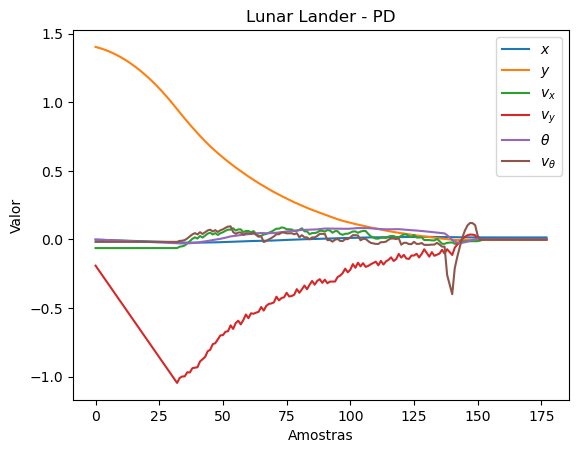
\includegraphics[scale=0.5]{llpid.png}
    \label{fig:llpid}
  \end{minipage}
  \begin{minipage}{0.5\textwidth}
    \centering
     \caption{GPC: \textit{Lunar Lander}.}
     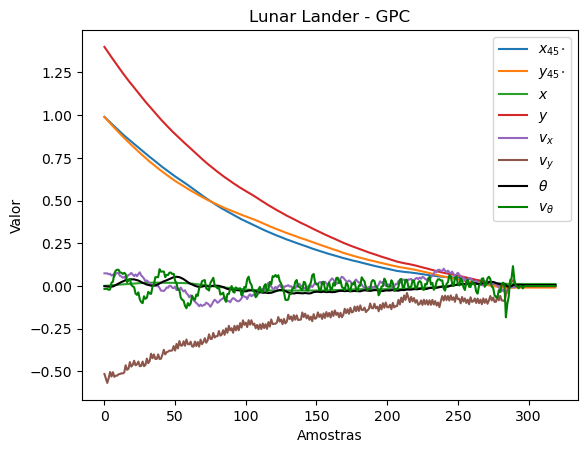
\includegraphics[scale=0.5]{llgpc.png}
    \label{fig:imagem2}
  \end{minipage}
\end{figure}
\vspace*{-1.2cm}
{\raggedright \fonte{Autor.}}

O GPC e o PD conseguiram realizar a aterrissagem da sonda lunar (\textit{Lunar Lander}). Observando o GIF dos dois pousos (Figura \ref{fig:pct} e \ref{fig:gct}) e o gráfico apresentado na Figura \ref{fig:llpid}, é evidente que o GPC adota uma abordagem mais cautelosa em comparação com o PD. Isso é perceptível pelo fato de o GPC iniciar a desaceleração da sonda antes do PD, resultando em um pouso mais suave, embora com mais etapas. Para validar foram considerados 1000 tentativas de pouso conforme mostrado na Tabela \ref{tab:outll}.

\begin{table}[H]
	\centering
	\vspace*{-.2cm}
	\caption{PID x GPC - \textit{Lunar Lander}.}
	\begin{tabular}{|c|c|c|c|c|c|}
			\hline
             Controle & Pouso & Pouso com +200 pontos & Etapas & Tempo de execução [$s$] & Pontuação média\\
            \hline
            PD & $765$ & $764$ &  $177577$ & $1086,6976$ & $217,4862$\\
            \hline
            GPC & $870$ & $808$  &  $340369$ & $1017,0346$ & $209,1881$\\ 
            \hline
	\end{tabular}  
    \label{tab:outll}                 % Nome da tabela para referência cruzada
\end{table}
\vspace*{-0.7cm}
{\raggedright \fonte{Autor.}}

De maneira geral, ambos os controladores obtiveram resultados satisfatórios, porém o GPC demonstrou superioridade em relação ao PD, apresentando uma resposta mais consistente em termos de episódios resolvidos (+200 pontos). Por exemplo, o GPC alcançou sucesso em $87\%$ das tentativas, indicando que a sonda conseguiu atingir o local de pouso designado e parou sem movimentos adicionais. Além disso, em $80,8\%$ das vezes, o GPC alcançou 200 pontos, indicando não apenas um pouso bem-sucedido, mas também a satisfação de outros critérios estabelecidos pelo ambiente para resolver completamente o desafio. Ao considerar um horizonte de predição igual a 4 ($H_p=4$) e um horizonte de controle igual a 2 ($H_c=2$), o GPC apresentou um tempo de execução melhor entre as amostras (0,6145 ms). No entanto, os PDs mostraram uma resposta de pontuação média melhor, pois, por serem mais arrojados em seus \textit{setpoints}, conseguiram pousar com menos amostras e acionamentos dos propulsores (principal e secundário).

Entretanto, neste caso, tratava-se de um sistema MIMO, o que exigia dois PDs aplicados de forma empírica, sem a utilização de um modelo matemático de caixa branca, como no caso do \textit{Cart Pole}. Tentou-se aplicar tal abordagem, mas a complexidade em determinar as relações entre as saídas e entradas, bem como estimar os parâmetros físicos da sonda por meio de simulações, revelou-se muito grande. Também foi observada uma dificuldade em definir um \textit{setpoint} mais elaborado para os PDs, optando-se por técnicas que simplificam os \textit{setpoints} para torná-los mais compatíveis com o controlador. Além disso, sua resposta não é aplicável, pois o \textit{Lunar Lander} opera com entradas inteiras, requerendo ajustes na saída dos PDs.

Por outro lado, o GPC utiliza um modelo ARX. Embora seja caixa preta, é mais flexível do ponto de vista da implementação de \textit{setpoints}, permitindo a inserção intuitiva de vários \textit{setpoints}. Outra vantagem é que ele fornece diretamente a ação de controle para o sistema.\\

%%%%%%%%%%%%%%%%%%%%%%%%%%%%%% CONCLUSÕES (OBRIGATÓRIO) %%%%%%%%%%%%%%%%%%%%%%%%%%%%%%

{\let\clearpage\relax\par \chapter{CONCLUSÕES}}
\label{ch:conclusoes}                       % Nome do capítulo para referência cruzada


Os resultados encontrados neste trabalho evidenciaram que ambas as técnicas de controle, tanto o Controle Proporcional-Integral-Derivativo quanto o Controle Preditivo Generalizado, demonstraram ser totalmente capazes de controlar sistemas complexos. É importante ressaltar que ambas as técnicas apresentaram desafios durante a implementação. Por exemplo, no caso do PID no \textit{Cart Pole} os parâmetros intrínsecos do sistema, como a massa do carro, do pêndulo e a altura da haste do pêndulo, utilizados na Função de Transferência, foram determinados empiricamente. No entanto, após a sintonização pelo GEKKO, o sistema controlado apresentou resultados altamente promissores.

Para implementar os PDs no \textit{Lunar Lander}, inicialmente planejou-se seguir os passos adotados no \textit{Cart Pole}. No entanto, a obtenção da Função de Transferência revelou-se custosa devido ao sistema ser MIMO (Múltiplas Entradas e Múltiplas Saídas). Além disso, a determinação dos parâmetros intrínsecos do sistema por experimentação mostrou-se inviável. Assim, optou-se por uma abordagem mais empírica, semelhante à aplicação industrial de controladores PID, onde muitos deles vêm com funcionalidades de ajuste automático incorporadas. No entanto, neste trabalho, o algoritmo de Subida de Encosta foi utilizado para ajustar os parâmetros conforme a recompensa, resultando em um bom controle.

A implementação do controle preditivo generalizado foi auxiliada pelo pacote SysIdentPy, uma ferramenta eficiente para identificação de sistemas. Um dos maiores desafios na identificação foi em relação ao \textit{Cart Pole}, onde mesmo com o auxílio do PRBS, foi necessário fixar o número de passos em dois milhões para obter o modelo com o maior episódio. Este problema foi atribuído à natureza instável do sistema, no entanto, o controle do \textit{Cart Pole} foi efetuado com sucesso. No \textit{Lunar Lander}, o SysIdentPy obteve ótimos modelos com poucas amostras, e os ajustes dos pesos na função custo foram realizados por meio de tentaiva e erro e com auxílio algoritmo de Subida de Encosta. O resultado atendeu aos objetivos estabelecidos.

Um dos principais obstáculos na implementação do GPC foi lidar com um problema de otimização inteira, que foi resolvido pelo Método de Pesquisa em Grade, um algoritmo com complexidade $O(n!)$, ou seja, o tempo de execução aumenta fatorialmente em relação à entrada. De maneira geral, no \textit{Cart Pole}, o PID, além de mais estável, foi mais rápido. Pois um dos seus problemas foi por ser um sistema instável, adotou-se um horizonte de controle igual ao de predição ($H_c=H_p=4$), o que aumenta a complexidade do algoritmo. Já no \textit{Lunar Lander}, a adoção de uma metodologia em termos de $u$ ao invés de $\Delta u$, permitiu otimizar a resposta em relação a pontuação. Além disso, o GPC demonstrou um tempo de resposta mais ágil em comparação ao controlador PID.


Em resumo, tanto o método PID quanto o MPC demonstraram capacidade de controlar sistemas complexos, como evidenciado no trabalho de Prata et al. em 2020 \cite{prata2020}, que sugere que um PID devidamente parametrizado pode rivalizar em desempenho com o MPC. No entanto, o PID apresentou melhor desempenho no controle do \textit{Cart Pole}, enquanto o GPC se destacou no controle do \textit{Lunar Lander}. Este estudo contribui para a compreensão e aplicação prática dessas técnicas em diferentes contextos, conforme observado por Taketa et al. em 2018 \cite{taketa2018}, abrindo caminho para futuras investigações e avanços neste campo promissor.\\

%%%%%%%%%%%%%%%%%% PROPOSTAS DE TRABALHOS FUTUROS (OBRIGATÓRIO) %%%%%%%%%%%%%%%%%%%%%%

{\let\clearpage\relax\par \chapter{PROPOSTAS DE TRABALHOS FUTUROS}}
\label{ch:propostas}                        % Nome do capítulo para referência cruzada


Segue abaixo uma lista de sugestões para os próximos trabalhos:

\begin{itemize}
\item Trabalhar com bibliotecas de otimização inteira em Python em conjunto com o Controle Preditivo Generalizado, como a Python-MIP, e comparar os resultados obtidos através do Método de Pesquisa em Grade em relação ao tempo de execução e pontuação;
\item Comparação de algoritmos de otimização para ajuste de parâmetros em controladores PID e GPC, incluindo algoritmos genéticos e de enxame de partículas.
\end{itemize}

%%%%%%%%%%%%%%%%%%%%%%%%%%%%%% BIBLIOGRAFIA (OBRIGATÓRIO) %%%%%%%%%%%%%%%%%%%%%%%%%%%%%%

\bibliographystyle{ieeetr}                  % Tipo de bibliografia utilizada
\bibliography{bibliografia}                 % Nome do arquivo .bib contendo a referência bibliográfica
			
%%%%%%%%%%%%%%%%%%%%%%%%%%%%%% FIM %%%%%%%%%%%%%%%%%%%%%%%%%%%%%%%%%%%%%%%%%%%%%%%%%
		
\end{OnehalfSpace}                          % Término do espaçamento de 1,5
\label{lastpage}
\end{document}